% =====================================================================
%  M.Sc. Thesis Proposal -- Armin Khalilzadeh
%  Sharif University of Technology, Graduate School of Management and Economics
%  Compile: pdflatex proposal.tex (x2)
% =====================================================================
\documentclass[11pt,a4paper]{article}

% ---------- Fonts & encoding ----------
\usepackage[T1]{fontenc}
\usepackage[utf8]{inputenc}
\usepackage[sc]{mathpazo}
\linespread{1.06}
\usepackage[scaled=0.90]{helvet}
\usepackage[final]{microtype}
\usepackage{needspace}

% ---------- Layout ----------
\usepackage[a4paper,top=2.6cm,bottom=2.6cm,left=2.75cm,right=2.75cm,headheight=14pt]{geometry}
\usepackage{setspace}
\setlength{\parskip}{0.42em}
\setlength{\parindent}{0pt}

% ---------- Math ----------
\usepackage{amsmath,amssymb,mathtools,bm}

% ---------- Colour, graphics, tables ----------
\usepackage[dvipsnames,table]{xcolor}
\definecolor{navy}{HTML}{1F3A5F}
\definecolor{steel}{HTML}{4A6F96}
\definecolor{mist}{HTML}{EEF2F7}
\definecolor{sand}{HTML}{F6EFE2}
\definecolor{rust}{HTML}{A44A3F}
\definecolor{ink}{HTML}{222222}
\definecolor{rule}{HTML}{B7C3D0}
\usepackage{graphicx}
\usepackage{booktabs,tabularx,threeparttable,makecell,multirow,array}
\usepackage{caption,subcaption}
\captionsetup{font={small},labelfont={bf,sf,color=navy},textfont={},
              labelsep=period,justification=justified,singlelinecheck=true}
\captionsetup[table]{position=top,skip=6pt}
\usepackage{enumitem}
\setlist{itemsep=2pt,topsep=4pt,parsep=0pt,leftmargin=1.4em}
\usepackage[most]{tcolorbox}
\usepackage{tikz}
\usetikzlibrary{positioning,arrows.meta,shapes.geometric,fit,calc,backgrounds}

% ---------- Section styling ----------
\usepackage{titlesec}
\titleformat{\section}{\sffamily\Large\bfseries\color{navy}}{\thesection}{0.8em}{}[\vspace{-0.3em}{\color{rule}\titlerule[0.6pt]}]
\titleformat{\subsection}{\sffamily\large\bfseries\color{navy}}{\thesubsection}{0.7em}{}
\titleformat{\subsubsection}{\sffamily\normalsize\bfseries\color{steel}}{\thesubsubsection}{0.6em}{}
\titleformat{\paragraph}[runin]{\sffamily\normalsize\bfseries\color{navy}}{}{0pt}{}[.]
\titlespacing*{\section}{0pt}{1.6em}{0.9em}
\titlespacing*{\subsection}{0pt}{1.2em}{0.4em}
\titlespacing*{\subsubsection}{0pt}{0.9em}{0.25em}
\titlespacing*{\paragraph}{0pt}{0.6em}{0.6em}

% ---------- Header / footer ----------
\usepackage{fancyhdr}
\pagestyle{fancy}
\fancyhf{}
\fancyhead[L]{\sffamily\footnotesize\color{steel}A.~Khalilzadeh \textperiodcentered{} M.Sc.\ Thesis Proposal}
\fancyhead[R]{\sffamily\footnotesize\color{steel}Spatial and Interpersonal Inequality in Iran}
\fancyfoot[C]{\sffamily\footnotesize\color{steel}\thepage}
\renewcommand{\headrulewidth}{0.4pt}
\renewcommand{\headrule}{\hbox to\headwidth{\color{rule}\leaders\hrule height \headrulewidth\hfill}}

% ---------- References & links ----------
\usepackage[authoryear,round]{natbib}
\setlength{\bibsep}{3pt}
\renewcommand{\bibfont}{\small}
\usepackage[hidelinks]{hyperref}
\hypersetup{colorlinks=true,linkcolor=navy,citecolor=steel,urlcolor=steel,
  pdftitle={Spatial and Interpersonal Inequality in Iran: M.Sc. Thesis Proposal},
  pdfauthor={Armin Khalilzadeh}}
\usepackage[capitalise,noabbrev]{cleveref}

% ---------- Convenience macros ----------
\newcommand{\SH}[2]{#1~SH\,(#2)}          % Solar Hijri year with Gregorian equivalent
\newcommand{\sh}{\textsc{sh}}
\newcommand{\E}{\mathbb{E}}
\newcommand{\Var}{\operatorname{Var}}
\newcommand{\Cov}{\operatorname{Cov}}
\newcommand{\NTL}{\textsc{ntl}}
\newcommand{\GDP}{\textsc{gdp}}

\newtcolorbox{keybox}[1][]{enhanced,breakable,colback=mist,colframe=navy,boxrule=0pt,
  leftrule=2.4pt,arc=0pt,outer arc=0pt,left=9pt,right=9pt,top=6pt,bottom=6pt,
  fonttitle=\sffamily\bfseries\color{navy},coltitle=navy,colbacktitle=mist,
  attach title to upper={\par\smallskip},#1}
\newtcolorbox{notebox}[1][]{enhanced,breakable,colback=sand,colframe=rust,boxrule=0pt,
  leftrule=2.4pt,arc=0pt,outer arc=0pt,left=9pt,right=9pt,top=6pt,bottom=6pt,
  fonttitle=\sffamily\bfseries\color{rust},coltitle=rust,colbacktitle=sand,
  attach title to upper={\par\smallskip},#1}

\begin{document}

% =====================================================================
%  TITLE PAGE
% =====================================================================
\pagenumbering{roman}
\begin{titlepage}
\thispagestyle{empty}
\centering
\vspace*{0.4cm}

\includegraphics[width=2.9cm]{figs/sharif_logo.png}\\[0.7cm]
{\sffamily\large\bfseries\color{navy} Sharif University of Technology}\\[0.15cm]
{\sffamily\normalsize\color{steel} Graduate School of Management and Economics}\\[1.6cm]
{\sffamily\small\scshape\color{steel} Master of Science Thesis Proposal \,$\cdot$\, Economics}\\[0.55cm]
{\color{rule}\rule{0.82\textwidth}{0.6pt}}\\[0.55cm]
{\LARGE\bfseries\color{navy} Places and People:\\[0.25cm]
\Large The Evolution of Spatial Inequality in Iran\\ and Its Relation to Interpersonal Inequality}\\[0.45cm]
{\large\itshape Evidence from Provincial GDP, Nighttime Lights,\\ and Satellite-Defined Cities, 1992--2024}\\[0.55cm]
{\color{rule}\rule{0.82\textwidth}{0.6pt}}\\[1.5cm]
\begin{tabular}{r@{\hspace{0.8em}}l}
{\sffamily\small\color{steel} Candidate} & {\large Armin Khalilzadeh}\\[0.2cm]
{\sffamily\small\color{steel} Supervisor} & {\large Dr.\ Saeed Tajrishy}\\[0.2cm]
{\sffamily\small\color{steel} Status} & {\large Proposal defended; thesis in progress}\\[0.2cm]
{\sffamily\small\color{steel} This version} & {\large English version, Aban 1405 SH \textperiodcentered{} November 2026}\\[0.2cm]
{\sffamily\small\color{steel} Code} & {\normalsize\href{https://github.com/arminkhalilzadeh/iran-ntl-regional-inequality}{github.com/arminkhalilzadeh/iran-ntl-regional-inequality}}
\end{tabular}
\vfill
{\footnotesize\color{steel}\sffamily
Years are reported in the Iranian Solar Hijri (SH) calendar used by all official statistics; a Solar year\\
begins on 21 March and is matched to the Gregorian year with which it overlaps most (e.g.\ 1383~SH $\approx$ 2004).}
\end{titlepage}

% =====================================================================
%  ABSTRACT
% =====================================================================
\thispagestyle{empty}
\begin{center}
{\sffamily\large\bfseries\color{navy} Abstract}
\end{center}
\vspace{-0.3em}
{\small
Economic inequality has two distinct faces: the dispersion of welfare across \emph{people} and the dispersion of economic activity across \emph{places}. Policies aimed at one need not move the other, yet Iran's distributional debate is conducted almost entirely through a single statistic, the national household Gini coefficient. This thesis builds what is, to my knowledge, the first long and methodologically consistent series of interprovincial spatial inequality for Iran (1371--1403~SH, 1992--2024), together with a satellite-defined system of Iranian cities, and compares the trajectory of both with interpersonal inequality.

The provincial series is anchored in official provincial GDP, which is available for a consistent 30-unit geography (Tehran and Alborz merged) over 1383--1401~SH. Following \citet{LessmannSeidel2017}, a calibration model linking GDP to nighttime lights (\NTL) with province fixed effects and a linear trend is estimated on this window and used to reconstruct GDP backward to 1371 and forward to 1403. The reconstructed series is the primary dataset because it is generated by a single method throughout; a measurement-error-weighted composite of official and light-based GDP, in the spirit of \citet{ChenNordhaus2011} and \citet{HendersonStoreygardWeil2012}, serves as the alternative. Parameter and residual uncertainty are propagated into confidence bands for every inequality index.

The second, and most novel, layer abandons administrative boundaries altogether. Following the urban-economics literature that delineates cities from contiguous lit areas \citep{Dingel2021,Harari2020}, urban footprints are drawn from VIIRS imagery after gas-flare masking, populated with a built-up--based population grid, and validated against independent settlement data. Between-city inequality, its decomposition into between- and within-province components, and the evolution of urban primacy then describe Iran's urban system from space.

Preliminary evidence supports the design: provincial GDP and total radiance are related with a cross-sectional elasticity of 0.996 ($R^2=0.67$), while the within-province temporal signal is weaker (two-way fixed-effects elasticity 0.36) and partly driven by gas-flaring provinces. This finding motivates the flare-masking, backcasting and uncertainty-propagation strategy. A first look at places versus people already shows that the two can diverge: between-province inequality in household expenditure rose from about 0.16 to 0.24 over 1391--1403~SH, while output-based inequality outside the flaring provinces showed no clear trend. The analysis is descriptive and comparative; it identifies periods of co-movement and divergence between the two dimensions of inequality and relates them to identifiable episodes such as the 1389~SH subsidy reform and the sanctions shocks.

\medskip
\noindent\textbf{Keywords:} spatial inequality; interpersonal inequality; nighttime lights; city delineation; measurement error; Iran.\\
\textbf{JEL:} D63, R11, R12, O18, C82.
}

\newpage
\setcounter{tocdepth}{2}
\begingroup\setlength{\parskip}{0pt}\small
\tableofcontents
\endgroup
\newpage
\pagenumbering{arabic}
\setcounter{page}{1}

% =====================================================================
\section{Introduction}\label{sec:intro}
% =====================================================================

Redistributive policy can be organised around two different targets. \emph{People-based} policies (cash transfers, targeted subsidies, social insurance, personal taxation) act directly on the distribution of income or consumption across households. \emph{Place-based} policies (regional development budgets, infrastructure programmes, industrial zones, fiscal decentralisation) act on the distribution of economic activity across territory. The two families are often justified by the same language of ``reducing inequality'', but they address different objects, and their outcomes must be measured with different instruments. The success of a people-based policy is naturally read off a household Gini coefficient; the success of a place-based policy requires a measure of how economic activity is distributed across regions.

The distinction matters most when the level at which a policy is targeted differs from the level at which it is evaluated. A national Gini that is stable or falling can coexist with widening gaps between provinces, because the national index aggregates within-region and between-region dispersion and the two components can move in opposite directions \citep{Shorrocks2005,Novotny2007}. Conversely, convergence of regional averages can coexist with deepening inequality within regions, for instance when selective out-migration of skilled workers raises measured income per capita in lagging regions while eroding their growth capacity \citep{Fratesi2014}. Recent work therefore argues that between-region and within-region inequality must be analysed jointly \citep{Rey2018,CapelloCerisola2024,LeeBreau2026}.

Why should spatial inequality be studied in its own right if the ultimate objective is the welfare of individuals? Three reasons stand out. First, place shapes opportunity: where a person is born and lives determines access to labour markets, education, health care and infrastructure, independently of her position in the national income distribution. Second, an unchanged national index can conceal a structural reallocation in which falling within-province dispersion offsets rising between-province gaps. Third, place-based interventions such as provincial development budgets leave only a faint trace in a national household index and can be evaluated credibly only with a measure defined at the same geographical scale.

Iran makes the question especially pressing. Chronic inflation, large relative-price swings, repeated sanctions shocks, an oil-dependent and spatially concentrated production structure, and a sizeable informal sector all affect households and regions through different channels. A universal cash-transfer programme, introduced with the 1389~SH (2010) subsidy reform, shifts household disposable income without altering where output is produced; sanctions act through trade, ports and export industries whose exposure is highly uneven across provinces. There is therefore no presumption that the two dimensions of inequality move together. Yet whereas the household Gini can be traced back to 1363~SH, there is no long and consistent series of spatial inequality: provincial accounts cover a limited span, administrative boundaries changed repeatedly, and the existing evidence relies on scattered years or on composite development indices.

\paragraph{What this thesis does}
The thesis constructs two new measures of spatial inequality and compares them with interpersonal inequality.
\begin{enumerate}[label=(\roman*)]
\item \emph{A provincial series, 1371--1403~SH.} Official provincial GDP for a fixed 30-unit geography over 1383--1401~SH is used to calibrate the GDP--\NTL{} relationship, which is then used to reconstruct GDP over the full period by a single, homogeneous method \citep{LessmannSeidel2017}. A measurement-error-weighted composite of official and light-based GDP is built as the alternative series, and uncertainty from the reconstruction is propagated into confidence bands for each index.
\item \emph{A satellite-defined city system.} Cities are delineated directly from nighttime lights rather than from official municipal or county (\emph{shahrestan}) boundaries, following the logic of \citet{Dingel2021} and \citet{Harari2020}. Between-city inequality in lights per capita, its decomposition into between- and within-province components, and the evolution of urban primacy describe the geography of Iran's urban economy.
\item \emph{A comparison of places and people.} Both spatial series are set against the national Gini coefficient to identify periods of co-movement, divergence and turning points, and to relate them to identifiable policy and macroeconomic episodes.
\end{enumerate}

The remainder of the proposal is organised as follows. \Cref{sec:rq} states the research questions and the testable implications that make the comparison informative. \Cref{sec:lit} reviews the literature. \Cref{sec:data} describes the data. \Cref{sec:prelim} reports preliminary evidence. \Cref{sec:method} sets out the methodology and econometric framework. \Cref{sec:validity} discusses threats to validity, robustness and limitations, and \cref{sec:contrib} summarises the expected contributions and the work plan.

% =====================================================================
\section{Motivation and Research Questions}\label{sec:rq}
% =====================================================================

\subsection{Two dimensions of inequality in Iran}

Interpersonal inequality in Iran has been anything but stable. According to the Statistical Centre of Iran (SCI), the national Gini coefficient of household expenditure (\cref{fig:gini}) fluctuated in a narrow band of 0.42--0.43 from 1363~SH until the mid-1380s, fell sharply in the late 1380s to a low of 0.365 in 1392~SH, rose again to 0.409 in 1397~SH, and has hovered around 0.39 in recent years. These movements show that individual inequality responded to macroeconomic and policy shocks, but by construction they say nothing about how the geographical distribution of economic activity evolved over the same period.

\begin{figure}[htbp]
\centering
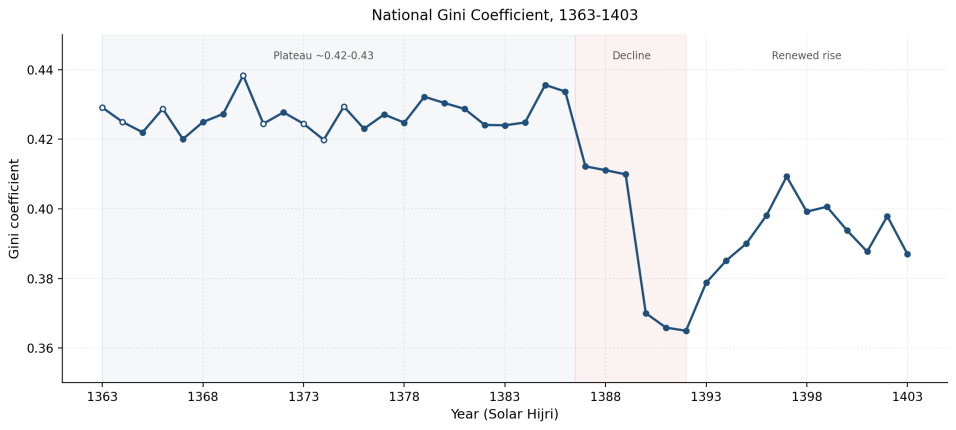
\includegraphics[width=0.94\textwidth]{figs/gini.png}
\caption{National Gini coefficient, 1363--1403~SH (1984--2024). Hollow markers denote early years computed without survey weights. Shaded areas mark the plateau, the decline around the 1389~SH subsidy reform, and the subsequent renewed rise. \emph{Source:} Statistical Centre of Iran.}
\label{fig:gini}
\end{figure}

The spatial side is equally uneven. Nighttime-light imagery shows that brightening since 1391~SH has not been spatially uniform: luminosity remains concentrated around the metropolitan cores, along a few industrial corridors, and in oil and gas regions (\cref{fig:maps}). Whether this concentration has increased or decreased, and whether it moved in step with household inequality, has not been established.

\begin{figure}[htbp]
\centering
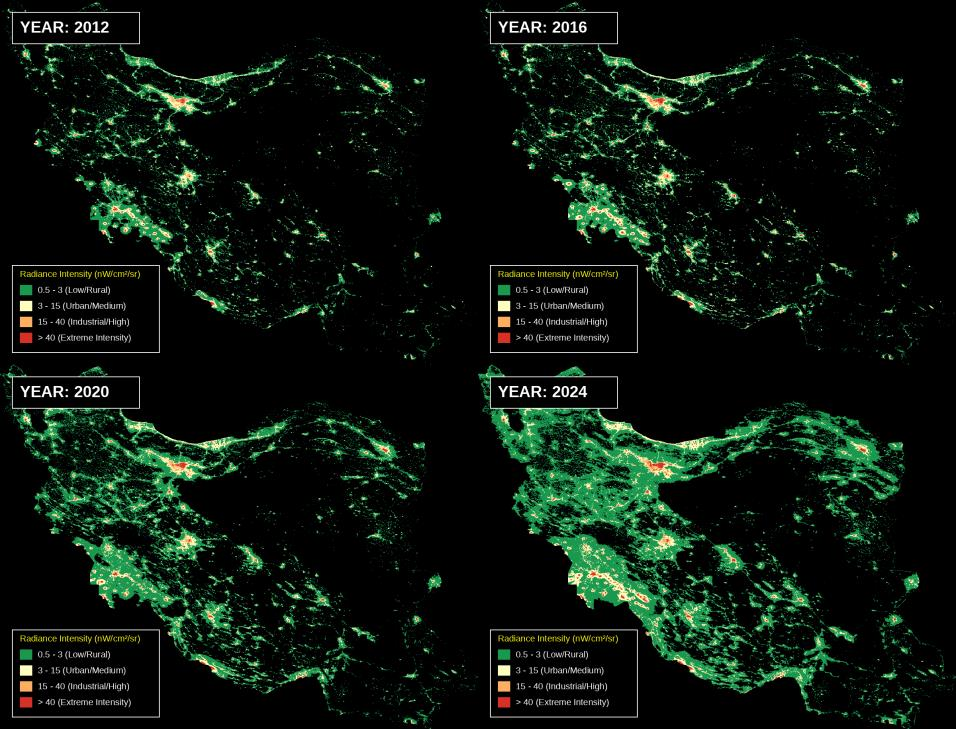
\includegraphics[width=0.86\textwidth]{figs/ntl_maps.png}
\caption{Nighttime radiance in Iran, 1391, 1395, 1399 and 1403~SH (2012, 2016, 2020, 2024). Colour classes from low/rural ($0.5$--$3$ nW\,cm$^{-2}$\,sr$^{-1}$) to extreme intensity ($>40$). \emph{Source:} author's processing of annual VIIRS composites.}
\label{fig:maps}
\end{figure}

\subsection{Research questions}

\begin{keybox}[title={Central question}]
How has the spatial inequality of economic activity in Iran evolved over the past three decades, and how does its trajectory compare with that of interpersonal inequality?
\end{keybox}

The central question is broken into three operational questions:

\begin{description}[leftmargin=0pt,labelindent=0pt,font=\sffamily\bfseries\color{navy}]
\item[RQ1 --- Provinces.] What is the trajectory of population-weighted interprovincial inequality in GDP per capita over 1371--1403~SH, once official data are extended with nighttime lights by a single, validated method, and how precisely can it be measured?
\item[RQ2 --- Cities.] When cities are defined by their lit footprint rather than by administrative boundaries, how unequal is Iran's urban system, how much of between-city inequality lies between rather than within provinces, and how has urban primacy evolved?
\item[RQ3 --- Places versus people.] Over which periods do spatial and interpersonal inequality move together or diverge, where are their turning points, and do the divergences align with episodes whose mechanisms predict them?
\end{description}

The analysis is descriptive and comparative. It does not seek to estimate a causal effect of one dimension on the other; the data provide no exogenous variation that could support such a claim, and the research question does not require one.

\subsection{Why the comparison is informative}

A comparison of two time series is informative only if theory gives reasons to expect them to diverge. The literature points to at least four mechanisms, each with an observable signature (\cref{tab:mechanisms}). Their existence turns the co-movement of the two series from a presumption into a testable proposition; establishing which pattern has dominated in Iran is part of the empirical contribution.

\begin{table}[htbp]
\centering\small
\caption{Mechanisms that can separate spatial from interpersonal inequality}
\label{tab:mechanisms}
\begin{tabularx}{\textwidth}{@{}>{\raggedright\arraybackslash}p{3.1cm}>{\raggedright\arraybackslash}X>{\raggedright\arraybackslash}p{4.1cm}@{}}
\toprule
\textbf{Mechanism} & \textbf{Logic} & \textbf{Observable signature}\\
\midrule
Selective migration & Skilled out-migration from lagging provinces narrows gaps in average income per capita while concentrating high earners in destination regions \citep{Fratesi2014}. & Spatial convergence with flat or rising interpersonal inequality.\\
\addlinespace
Composition of total inequality & The national Gini contains between- and within-region components that can offset each other \citep{Shorrocks2005,Novotny2007}. & Stable national Gini alongside a trending spatial index.\\
\addlinespace
Universal cash transfers & Transfers of equal absolute size raise the income share of poor households everywhere without moving the location of production. & Sharp fall in the Gini around 1389~SH with little change in spatial inequality.\\
\addlinespace
Sanctions and trade shocks & Exposure runs through ports, border trade and export industries and is spatially concentrated. & Movements in spatial inequality around 1390--91 and 1397~SH that exceed those in the Gini.\\
\bottomrule
\end{tabularx}
\end{table}

% =====================================================================
\section{Literature Review}\label{sec:lit}
% =====================================================================

The relevant literature is organised in six strands (\cref{fig:littree}): the theory of regional inequality; the relationship between spatial and interpersonal inequality; nighttime lights as a measure of economic activity and the logic of combining noisy signals; the measurement of regional inequality with lights; the delineation of cities from space; and the evidence on Iran. The research gap and the position of this thesis follow.

\begin{figure}[htbp]
\centering
\resizebox{\textwidth}{!}{%
\begin{tikzpicture}[
  font=\sffamily,
  root/.style={rectangle,rounded corners=3pt,fill=navy,text=white,font=\sffamily\bfseries\small,
               minimum width=8.6cm,minimum height=0.85cm,align=center},
  head/.style={rectangle,rounded corners=2pt,fill=steel,text=white,font=\sffamily\bfseries\scriptsize,
               text width=2.55cm,minimum height=1.0cm,align=center},
  newhead/.style={head,fill=rust},
  body/.style={rectangle,rounded corners=2pt,draw=rule,fill=mist,font=\sffamily\tiny,
               text width=2.55cm,align=center,inner sep=4pt,minimum height=2.45cm},
  newbody/.style={body,fill=sand,draw=rust!40},
  gap/.style={rectangle,rounded corners=3pt,fill=sand,draw=rust!60,font=\sffamily\scriptsize,
              text width=16.8cm,align=center,inner sep=6pt},
  ours/.style={rectangle,rounded corners=3pt,fill=navy,text=white,font=\sffamily\scriptsize,
               text width=16.8cm,align=center,inner sep=6pt},
  arr/.style={-{Stealth[length=2.2mm]},draw=steel,line width=0.6pt}]
\node[root] (root) at (0,0) {Spatial inequality and its measurement from space};
\foreach \i/\x/\t in {1/-7.15/{3.1\\Regional inequality:\\theory},
                      2/-4.29/{3.2\\Spatial vs.\\interpersonal},
                      3/-1.43/{3.3\\Lights as a measure;\\combining signals},
                      4/1.43/{3.4\\Regional inequality\\from lights}}
  {\node[head] (h\i) at (\x,-1.7) {\t};}
\node[newhead] (h5) at (4.29,-1.7) {3.5\\Delineating cities\\from space};
\node[head] (h6) at (7.15,-1.7) {3.6\\Evidence\\on Iran};
\node[body,below=0.12cm of h1] (b1) {Williamson (1965)\\Alonso (1980)\\Amos (1988)\\Krugman (1991)\\Magrini (2004)};
\node[body,below=0.12cm of h2] (b2) {Shorrocks \& Wan (2005)\\Novot\'y (2007)\\Fratesi \& Percoco (2014)\\Rey (2018)\\Capello \& Cerisola (2024)\\Lee \& Breau (2026)};
\node[body,below=0.12cm of h3] (b3) {Chen \& Nordhaus (2011)\\Henderson et al.\ (2012)\\Pinkovskiy \&\\Sala-i-Martin (2016)\\Gibson et al.\ (2021)\\Li et al.\ (2020)};
\node[body,below=0.12cm of h4] (b4) {Lessmann (2014)\\Lessmann \& Seidel (2017)\\Mveyange (2015)\\Mirza et al.\ (2021)\\Galimberti et al.\ (2023)};
\node[newbody,below=0.12cm of h5] (b5) {Small et al.\ (2005)\\Rozenfeld et al.\ (2011)\\Zhou et al.\ (2014)\\Harari (2020)\\Dingel et al.\ (2021)\\Bluhm \& Krause (2022)};
\node[body,below=0.12cm of h6] (b6) {Noorbakhsh (2005)\\Pourfaraj et al.\ (2019)\\Hadizadeh (2020)\\Farzanegan \&\\Fischer (2021)\\Fouladgar \& Feizi (2023)};
\foreach \i in {1,...,6}{\draw[arr] (root.south) -- ++(0,-0.45) -| (h\i.north);}
\node[gap] (gap) at (0,-6.25) {\textbf{3.7 Research gap.} No long, methodologically consistent series of spatial inequality exists for Iran; no study sets such a series against interpersonal inequality; and Iran's urban system has never been delineated independently of administrative boundaries.};
\foreach \i in {1,...,6}{\draw[arr] (b\i.south) -- (b\i.south |- gap.north);}
\node[ours,below=0.4cm of gap] (ours) {\textbf{This thesis.} A provincial spatial-inequality series for 1371--1403~SH calibrated on official GDP and extended with lights, with propagated uncertainty; a satellite-defined city system with between-city inequality; and a systematic comparison of both with the national Gini.};
\draw[arr] (gap.south) -- (ours.north);
\end{tikzpicture}}
\caption{Structure of the literature review and key contributions in each strand. The strand highlighted in rust underpins the city module.}
\label{fig:littree}
\end{figure}

\subsection{Regional inequality: theory and mechanisms}

The modern theory of regional inequality begins with \citet{Williamson1965}, who carried Kuznets' \citeyearpar{Kuznets1955} inverted-U hypothesis from the distribution of income across persons to the distribution across regions. In early development, growth starts in regions favoured by resources, location or infrastructure; capital and skilled labour flow towards them (``backwash'' effects) and regional gaps widen. Later, congestion costs, rising wages in the core and public investment in the periphery (``spread'' effects) favour convergence. The new economic geography offers a different equilibrium view: agglomeration economies arising from shared labour markets, input--output linkages and knowledge spillovers can make spatial concentration self-reinforcing even in advanced economies \citep{Krugman1991}, so that the inverted U is not guaranteed.

\citet{Alonso1980} generalised Williamson's argument into a family of ``bell-shaped'' curves (for interpersonal inequality, regional inequality, geographical concentration and demographic transition) and stressed that these dimensions are interdependent, so that analysing one in isolation is incomplete. \citet{Amos1988} showed for US states that regional inequality can rise again after the inverted U is completed, as structural change towards knowledge-intensive activities creates new sources of divergence. Finally, \citet{Magrini2004} showed that part of the contradictory evidence on regional convergence stems from differences in the definition of regions and in the level of aggregation, a reminder that the choice of spatial unit and measure is itself part of the result. This point motivates the second, city-based layer of the present thesis.

\subsection{Spatial versus interpersonal inequality}

Whether the spatial dimension carries information beyond interpersonal inequality is the central conceptual question. Decomposition studies show that between-region inequality typically accounts for a minority of total inequality \citep{Shorrocks2005,Novotny2007}, and \citet{AzamBhatt2018} document for India that within-district differences dominate even as the between-district share grows. \citet{Novotny2007} argues, however, that a small statistical share does not imply irrelevance: spatial disparities weigh heavily for social cohesion and political economy. The Gini coefficient is not additively decomposable: its decomposition leaves an overlap term that is rarely negligible, which is why the generalised-entropy family is preferred whenever decomposition is the objective.

On mechanisms, \citet{Fratesi2014} show for Italy that selective migration of educated workers from lagging to advanced regions produces apparent convergence in average income while undermining the long-run growth capacity of origin regions; the two dimensions can thus move in opposite directions. \citet{Rey2018} documents, for the United States, periods in which interregional and interpersonal inequality moved in opposite directions, and \citet{KhanSiddique2021} find that US regional inequality reached a historic low while income inequality peaked. \citet{LeeBreau2026}, using a two-stage Theil decomposition across three spatial scales for 1970--2020, show that the relevant scale itself shifts: between-state differences dominated interregional inequality in 1970, whereas inequality within local labour markets dominated by 2020. \citet{CapelloCerisola2024} provide the closest theoretical framework: a ``double bell'' in which inter- and intra-regional disparities evolve jointly, so that a decline in one is not evidence of distributive success if the other rises. Their framework justifies the joint analysis of the two time series in this thesis.

\subsection{Nighttime lights as a measure of activity and the logic of combining signals}

Nighttime lights proxy economic activity because production and consumption require artificial light at night. Their key virtue for measurement is that they are generated by a process entirely independent of national statistical systems, so that their errors are plausibly unrelated to those of official accounts. \citet{ChenNordhaus2011} framed official GDP and luminosity as two noisy measures of the same unobserved quantity: if their errors are independent, a weighted average has lower error variance than either, and lights add most value where statistical systems are weakest. \citet{HendersonStoreygardWeil2012} formalised this as a signal-extraction problem and derived optimal weights from the ratio of measurement-error variances, while \citet{PinkovskiySalaiMartin2016} used lights as an arbiter in the debate between national accounts and household surveys. These papers supply the theory behind the composite estimator used here as the alternative dataset (\cref{sec:datasetB}).

Two generations of sensors are relevant. The DMSP-OLS series (1992--2013) suffers from top-coding in bright cores, ``blooming'' of light into neighbouring pixels and inter-satellite calibration inconsistencies; the VIIRS series (from 2012) offers finer resolution, a wider dynamic range and on-board calibration \citep{Elvidge2021}. \citet{Gibson2021} show that DMSP's deficiencies can produce misleading results at fine spatial scales, and \citet{Gibson2025} review how blurring, top-coding and temporal inconsistency bias economic applications. Because blooming and saturation are partly absorbed when lights are summed over large units, these problems are much smaller at the provincial level than at the city level, and this shapes the sensor choices in \cref{sec:method}. Harmonised DMSP--VIIRS series \citep{Li2020,ChenZ2021} make long panels possible.

\subsection{Measuring regional inequality with nighttime lights}

\citet{Lessmann2014} tested the inverted-U relationship between regional inequality and development with regional income data for a broad set of countries. \citet{LessmannSeidel2017} replaced regional income with lights: they estimate the relationship between regional income and luminosity where both exist and use it to predict regional income everywhere, producing the first systematic cross-country dataset of light-based, population-weighted regional inequality. Their two-step logic is the backbone of the reconstruction in this thesis. \citet{Mveyange2015} applied the approach to Africa, where regional accounts are almost absent; \citet{Wu2018}, \citet{Singhal2020} and \citet{Ivan2020} did so for China, India and Romania respectively.

A related strand computes inequality directly from the spatial distribution of lights per capita. \citet{Mirza2021} derive Gini coefficients from lights per person and validate them against income inequality across countries and US states; \citet{WeidmannTheunissen2021} validate local light-based inequality against survey data; \citet{WeidmannSchutte2017} show that lights predict local wealth well; and \citet{Montalvo2021} discuss how saturation in bright areas can understate true inequality. \citet{Galimberti2023} draw a distinction that is crucial for a long time series: high cross-sectional correlation between lights and output does not imply that changes in lights track changes in output. Temporal validity must be assessed separately, a principle that underlies the validation design in \cref{sec:validation}.

\subsection{Delineating cities from space}\label{sec:litcities}

Administrative boundaries are a poor guide to the economic extent of cities: they cut through metropolitan areas, lump rural hinterlands with urban cores, and change over time. An established literature therefore defines urban areas from the contiguous extent of human activity observed from space.

\paragraph{Thresholding and contiguity}
The foundational approach classifies pixels whose luminosity exceeds a threshold as urban and treats contiguous lit pixels as one city. \citet{Imhoff1997} introduced the method on DMSP composites and showed that urban extent is highly sensitive to the threshold because of blooming; \citet{Small2005} documented the same sensitivity globally, showing that lit areas grow systematically larger than built-up areas at low thresholds. Because a single global threshold fits poorly across regions, \citet{Zhou2014} proposed cluster-specific thresholds calibrated against high-resolution urban maps.

\paragraph{Clustering algorithms}
\citet{Rozenfeld2008,Rozenfeld2011} introduced the City Clustering Algorithm, which builds cities bottom-up by merging populated cells within a given distance, independently of administrative units. Their results show that properties of the city-size distribution, such as Zipf's law, depend on how cities are defined, an observation that the economics literature later confirmed with lights.

\paragraph{Applications in economics}
\citet{Dingel2021} construct ``light-based metropolitan areas'' from contiguous areas brighter than a threshold (thresholds from 10 to 60 on the DMSP scale) and show that they match commuting-based metropolitan definitions closely in the United States and Brazil, whereas administrative units in China and India distort the city-size distribution; their conclusions are robust across thresholds, although urban fringes remain sensitive. \citet{Harari2020} uses DMSP-based footprints to measure city shape in India. \citet{ChMartinVargas2021} build a globally comparable measure of metropolitan size from stable lit pixels after correcting for blurring and inter-satellite comparability. \citet{Bluhm2022} show that lights can proxy city-level activity only after correcting top-coding, recovering the heavy-tailed distribution of ``top lights''. \citet{Abrahams2018} propose a deblurring procedure for DMSP footprints.

\paragraph{Alternatives and benchmarks}
Daytime imagery and building data offer independent benchmarks. \citet{Baragwanath2021} delineate Indian urban markets from built-up land cover and show that they are more numerous and cover more of the urban population than light-based markets. \citet{deBellefon2021} delineate French urban areas from building density, and the Degree of Urbanisation \citep{Dijkstra2021} defines urban centres from gridded population and built-up surfaces in a harmonised way across countries. These products are natural validation benchmarks for light-based footprints.

\paragraph{Population for satellite-defined units}
Satellite-defined cities require population counts that do not depend on administrative units. Gridded population products differ in construction \citep{Leyk2019}. WorldPop disaggregates census totals with a random-forest model whose covariates include VIIRS nighttime lights \citep{Stevens2015}; the GHS-POP grid allocates census totals in proportion to the volume of built-up surface \citep{Schiavina2023,Pesaresi2024}. For a measure such as lights per capita, a population grid built from lights would induce mechanical correlation, which is why a built-up--based grid is preferred here.

\subsection{Evidence on Iran}

\citet{Noorbakhsh2005} provided the first comprehensive analysis of spatial inequality and polarisation across Iranian provinces, finding substantial disparities and a cluster of deprived provinces whose gap was widening. \citet{Pourfaraj2019} measure provincial inequality with the Theil index and a population-weighted coefficient of variation for 2001--2015 and find significant spatial dependence. \citet{Hadizadeh2020} studies the convergence of provincial Gini coefficients and finds movement towards a common steady state of about 0.3. Persian-language studies test the inverted-U hypothesis with Williamson's index and spatial dynamic panels \citep{DehghanShabani2019} and analyse transition dynamics of a composite development index \citep{Ahmadi2019}; a decomposition of the national Gini by urban and rural areas shows that within-group inequality dominates \citep{Abounoori2013}. What these studies share is reliance on official data or composite indices, and none uses nighttime lights to reconstruct a long series.

Lights have been used for Iran for other questions. \citet{FarzaneganFischer2021} use harmonised lights for Iran's provinces over 1992--2018 to study the effect of sanctions relief on the shadow economy, showing both that provincial lights are usable over long horizons and that they capture activity not recorded in official GDP. \citet{FouladgarFeizi2023} use VIIRS to nowcast quarterly GDP over 1391--1399~SH: lights alone explain 83 per cent of the variation in non-oil GDP, 95 per cent with seasonal population and dummies, and out-of-sample errors for three quarters are below 2 per cent. This is direct evidence of the temporal validity of lights at the national level.

\subsection{Research gap and position of this thesis}\label{sec:gap}

Three streams have developed largely in isolation: the theory of development and regional inequality, the measurement of regional activity from space, and the comparison of spatial and interpersonal inequality. The gap is not the absence of either light-based regional inequality measures or comparisons of the two dimensions (both literatures exist) but their connection, and the specific situation of Iran.

\begin{keybox}[title={Research gap}]
\begin{enumerate}[label=\arabic*.,leftmargin=1.2em]
\item No long and methodologically consistent series of interprovincial inequality in economic activity exists for Iran; existing studies cover scattered years, the years with published accounts, or composite indices.
\item No study sets a spatial-inequality series for Iran against interpersonal inequality. The closest precedents are \citet{Rey2018} for the United States and \citet{CapelloCerisola2024} for Europe, neither of which concerns an oil-dependent developing economy with a centralised institutional structure and repeated external shocks.
\item To the author's knowledge, Iran's urban system has never been delineated independently of administrative boundaries, so inequality across Iranian cities as economic entities is unmeasured.
\end{enumerate}
\end{keybox}

Methodologically, most light-based studies treat lights as an error-free substitute for output. This thesis keeps official GDP as the anchor, treats both sources as noisy, tests the temporal stability of the calibration explicitly, and carries reconstruction uncertainty through to the inequality indices.

% =====================================================================
\section{Data}\label{sec:data}
% =====================================================================

\subsection{Sources}

\Cref{tab:sources} summarises the data. Four blocks are used: official accounts, nighttime lights, interpersonal inequality, and population and auxiliary layers.

\begin{table}[htbp]
\centering\small
\caption{Data sources}
\label{tab:sources}
\begin{tabularx}{\textwidth}{@{}>{\raggedright\arraybackslash}p{2.9cm}>{\raggedright\arraybackslash}X>{\raggedright\arraybackslash}p{2.15cm}>{\raggedright\arraybackslash}p{2.9cm}@{}}
\toprule
\textbf{Variable} & \textbf{Description and role} & \textbf{Coverage} & \textbf{Source}\\
\midrule
\multicolumn{4}{@{}l}{\textit{Official accounts}}\\
Provincial GDP & Constant 1400 prices; total and non-oil. Calibration and validation anchor. & 1383--1401~SH & SCI\\
National GDP & Quarterly, total and non-oil; national validation. & 1391--1403~SH & SCI / CBI\\
\addlinespace
\multicolumn{4}{@{}l}{\textit{Nighttime lights}}\\
VIIRS annual (VNL v2) & 15 arc-second radiance, nW\,cm$^{-2}$\,sr$^{-1}$; main source from 1391~SH and for cities. & 1391--1403~SH & \citet{Elvidge2021}\\
Harmonised series & DMSP--VIIRS consistent series for the pre-VIIRS years. & 1371--1401~SH & \citet{Li2020}; \citet{ChenZ2021}\\
Gas flares & Flare-site locations for pixel-level masking. & 1391~SH-- & \citet{Elvidge2016}\\
\addlinespace
\multicolumn{4}{@{}l}{\textit{Interpersonal inequality}}\\
National Gini & Household expenditure Gini from the HIES. & 1363--1403~SH & SCI\\
\addlinespace
\multicolumn{4}{@{}l}{\textit{Population and auxiliary layers}}\\
Provincial population & Censuses (1385, 1390, 1395) and intercensal estimates. & 1371--1403~SH & SCI\\
GHS-POP & 100\,m population grid allocated by built-up volume; main source for cities. & 5-year epochs 2005--2025 & \citet{Schiavina2023}\\
WorldPop & 100\,m grid (uses lights as a covariate); robustness only. & 2000--2020 & \citet{Stevens2015}\\
GHSL urban centres & Degree-of-Urbanisation centres; validation of city footprints. & 5-year epochs & \citet{Dijkstra2021}\\
Electricity consumption & Provincial consumption; third indicator for error variances. & 1383--1401~SH$^{\ddagger}$ & Ministry of Energy\\
Gridded GDP & Independent external comparator for reconstructed provincial GDP. & 2012-- & \citet{RossiHansbergZhang2025}\\
\bottomrule
\end{tabularx}
\begin{minipage}{\textwidth}\footnotesize\smallskip
\emph{Notes:} SCI = Statistical Centre of Iran; CBI = Central Bank of Iran; HIES = Household Income and Expenditure Survey. All lights data are extracted on Google Earth Engine. Early Gini values are unweighted, which is taken into account when interpreting levels. $^{\ddagger}$To be compiled from Ministry of Energy statistical yearbooks.
\end{minipage}
\end{table}

\subsection{Panel structure, geography and time}\label{sec:panel}

The provincial panel has 30 units observed annually over 1371--1403~SH. The geography is fixed at the post-1383 map, the year in which Khorasan was divided into North, Razavi and South Khorasan. The only later change, the creation of Alborz from Tehran in 1389~SH, is undone by merging the two provinces into a single unit, so that every unit has a constant territory throughout the period. Because nighttime lights are gridded, they can be summed over the fixed polygons for any year, including years before the units existed administratively. This is what allows province fixed effects to be estimated and used for prediction outside the calibration window.

The period divides into three segments, summarised in \cref{fig:timeline}:
\begin{itemize}
\item \emph{Calibration window, 1383--1401~SH} (2004--2022): official GDP and lights both observed; $30\times 19=570$ province-years.
\item \emph{Backcast, 1371--1382~SH} (1992--2003): lights only; GDP reconstructed.
\item \emph{Forecast, 1402--1403~SH} (2023--2024): lights only; GDP reconstructed.
\end{itemize}
The comparison with interpersonal inequality covers 1371--1403~SH, so that the Gini and spatial series share the same span; Gini values before 1371 are shown only as historical context.

\begin{figure}[htbp]
\centering
\begin{tikzpicture}[font=\sffamily\scriptsize,x=0.41cm,y=1cm]
  % x coordinate = Solar year minus 1371
  \draw[rule,line width=0.6pt] (0,0) -- (32.6,0);
  \foreach \y in {1371,1375,1379,1383,1387,1391,1395,1399,1403}{
     \draw[rule] ({\y-1371},0.08) -- ({\y-1371},-0.08);
     \node[below,text=steel] at ({\y-1371},-0.08) {\y};}
  % provincial segments
  \fill[steel!25] (0,0.35) rectangle (11.95,0.95);  \node[text=navy] at (6,0.65) {Backcast (lights only)};
  \fill[navy] (12,0.35) rectangle (30.95,0.95);      \node[text=white] at (21.5,0.65) {Calibration window: official GDP + lights};
  \fill[steel!25] (31,0.35) rectangle (32.95,0.95);  \node[text=navy] at (32,1.18) {Forecast};
  % sensors
  \fill[rust!25] (0,1.55) rectangle (20.95,2.05);    \node[text=rust!80!black] at (10.5,1.8) {DMSP-OLS (harmonised)};
  \fill[rust!60] (20,2.2) rectangle (32.95,2.7);     \node[text=white] at (26.5,2.45) {VIIRS};
  % cities
  \draw[navy,line width=1.6pt,-{Stealth[length=2mm]}] (20,3.2) -- (32.95,3.2) node[pos=0.5,above,text=navy] {City module (main)};
  \draw[navy,dashed,line width=1pt] (12,3.2) -- (20,3.2) node[pos=0.5,above,text=steel] {extension};
  % gini
  \draw[ink,line width=0.8pt] (0,-0.95) -- (32.95,-0.95) node[pos=0.5,below,text=ink] {National Gini (HIES): comparison period};
  % 1389 reform marker
  \draw[rust,dashed] (18,-0.6) -- (18,2.95);
  \node[text=rust,font=\sffamily\tiny,align=center,fill=white,inner sep=1pt] at (17.2,1.18) {1389 subsidy reform};
  % labels at left
  \node[anchor=east,text=steel,font=\sffamily\tiny] at (-0.3,0.65) {Provinces};
  \node[anchor=east,text=steel,font=\sffamily\tiny] at (-0.3,2.1) {Sensors};
  \node[anchor=east,text=steel,font=\sffamily\tiny] at (-0.3,3.2) {Cities};
  \node[anchor=east,text=steel,font=\sffamily\tiny] at (-0.3,-0.95) {People};
\end{tikzpicture}
\caption{Time structure of the analysis. The provincial geography is fixed at the post-1383 map with Tehran and Alborz merged (30 units).}
\label{fig:timeline}
\end{figure}

\subsection{Variables}

Monetary variables are expressed in constant 1400 prices. Lights for unit $i$ and year $t$ are measured as total (summed) radiance $L_{it}$; mean radiance and lights per capita are used descriptively. Regressions use logarithms, which make distributions more symmetric and give coefficients an elasticity interpretation. Total rather than per-capita quantities enter the calibration regression, so that a common population denominator does not create spurious correlation. Satellite data are mapped from the Gregorian to the Solar calendar by maximum temporal overlap, and province names across sources are reconciled through a standard code table.

\Cref{tab:summary} reports summary statistics for the preliminary sample assembled so far (31 provinces under current divisions, VIIRS years). The mean exceeds the median for every variable, reflecting right skew and the concentration of activity in a few provinces; the final panel will be rebuilt on the 30-unit geography and extended to the full calibration window.

\begin{table}[htbp]
\centering\small
\caption{Summary statistics, preliminary sample}
\label{tab:summary}
\begin{threeparttable}
\setlength{\tabcolsep}{4.2pt}\footnotesize
\begin{tabular}{@{}lcrrrrrr@{}}
\toprule
Variable & Period (SH) & $N$ & Mean & S.D. & Min & Median & Max\\
\midrule
Total radiance$^{a}$ & 1391--1403 & 403 & 64{,}170.8 & 75{,}831.7 & 9{,}335.8 & 39{,}385.7 & 595{,}551.1\\
Mean radiance & 1391--1403 & 403 & 1.595 & 1.726 & 0.146 & 0.948 & 7.909\\
Radiance per capita & 1391--1403 & 403 & 0.0320 & 0.0329 & 0.0057 & 0.0188 & 0.1727\\
Population (million) & 1391--1403 & 403 & 2.63 & 2.50 & 0.56 & 1.77 & 14.43\\
Provincial GDP (trillion rials) & 1390--1400 & 341 & 2{,}610.1 & 3{,}872.1 & 253.6 & 1{,}349.9 & 19{,}586.5\\
GDP per capita (million rials) & 1390--1400 & 341 & 1{,}035.5 & 1{,}071.1 & 228.5 & 676.5 & 6{,}982.2\\
\bottomrule
\end{tabular}
\begin{tablenotes}\footnotesize
\item \emph{Notes:} $^{a}$Radiance in nW\,cm$^{-2}$\,sr$^{-1}$. 31 provinces under current administrative divisions; monetary values in constant 1400 prices. Differences in $N$ reflect source coverage. \emph{Source:} author's calculations from SCI data and VIIRS imagery.
\end{tablenotes}
\end{threeparttable}
\end{table}

% =====================================================================
\section{Preliminary Evidence}\label{sec:prelim}
% =====================================================================

Part of the empirical work has been completed. Its purpose is to show that the approach is feasible and to document the facts on which the design rests. All results below use the preliminary 31-province sample and VIIRS years; they will be re-estimated on the final 30-unit panel and the full calibration window.

\subsection{National validation}

Using quarterly data (51 quarters), the elasticity of national GDP with respect to total radiance is 0.239 ($R^2=0.544$) and that of non-oil GDP is 0.246 ($R^2=0.493$), both significant at 1 per cent (\cref{tab:national}). The near-identical elasticities matter: if lights mainly recorded oil-related flaring, the elasticity for non-oil output would be much smaller. The simple correlations are 0.738 and 0.702 (\cref{fig:national}).

\begin{table}[htbp]
\centering\small
\begin{minipage}[t]{0.44\textwidth}
\vspace{0pt}
\captionof{table}{National validation (quarterly)}
\label{tab:national}
\setlength{\tabcolsep}{4pt}
\begin{tabular}{@{}lcc@{}}
\toprule
 & \multicolumn{2}{c}{Dep.\ var.: log GDP}\\
\cmidrule(l){2-3}
 & (1) & (2)\\
 & Total & Non-oil\\
\midrule
Log total radiance & 0.239$^{***}$ & 0.246$^{***}$\\
                   & (0.031) & (0.036)\\
Constant & 13.961$^{***}$ & 13.609$^{***}$\\
         & (0.386) & (0.441)\\
\midrule
Observations & 51 & 51\\
$R^2$ & 0.544 & 0.493\\
$F$-statistic & 58.55 & 47.65\\
\bottomrule
\end{tabular}

\smallskip
{\footnotesize Standard errors in parentheses. $^{***}p<0.01$.}
\end{minipage}\hfill
\begin{minipage}[t]{0.53\textwidth}
\vspace{0pt}
\centering
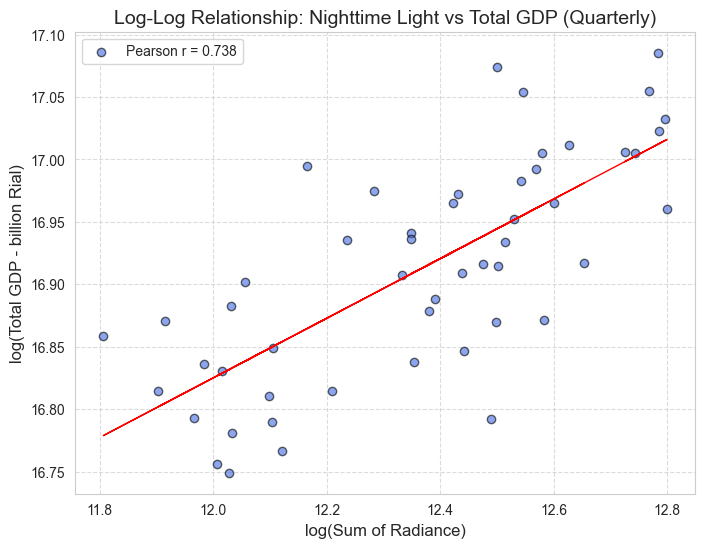
\includegraphics[width=\textwidth]{figs/national_scatter.png}
\captionof{figure}{Log total radiance and log total GDP, quarterly.}
\label{fig:national}
\end{minipage}
\end{table}

\subsection{Provincial validation: levels and within-province variation}\label{sec:prelimprov}

\Cref{tab:provincial} reports the provincial relationship. In the pooled cross-section (column 1), the elasticity of total provincial GDP with respect to total radiance is 0.996 (s.e.\ 0.040), essentially one-for-one, with $R^2=0.674$ and a correlation of 0.821. Since both variables scale with the size of the provincial economy, a near-proportional relationship is expected in levels.

The within-province temporal relationship is the more demanding test, because it is what the reconstruction relies on outside the calibration window. With province and year fixed effects (column 2), the elasticity falls to 0.361 and remains significant ($p=0.014$); the correlation between GDP and lights net of both sets of fixed effects is 0.431 ($p<0.001$). When the four provinces most affected by gas flaring (Bushehr, Khuzestan, Ilam and Kohgiluyeh and Boyer-Ahmad) are excluded (column 3), the elasticity falls further to 0.227 and loses significance.

\begin{table}[htbp]
\centering\small
\caption{Provincial validation: log GDP on log total radiance, 1391--1400~SH}
\label{tab:provincial}
\begin{threeparttable}
\begin{tabular}{@{}lccc@{}}
\toprule
 & (1) & (2) & (3)\\
 & Pooled OLS & Two-way FE & Two-way FE,\\
 &  &  & excl.\ flare provinces\\
\midrule
Log total radiance & 0.996$^{***}$ & 0.361$^{**}$ & 0.227\\
 & (0.040) & [$p=0.014$] & [n.s.]\\
\midrule
Province fixed effects & No & Yes & Yes\\
Year fixed effects & No & Yes & Yes\\
Provinces & 31 & 31 & 27\\
Observations & 310 & 310 & 270\\
$R^2$ & 0.674 & -- & --\\
Correlation of GDP and lights & 0.821 & 0.431$^{\dagger}$ & --\\
\bottomrule
\end{tabular}
\begin{tablenotes}\footnotesize
\item \emph{Notes:} Standard error in parentheses; $p$-values in brackets. $^{***}p<0.01$, $^{**}p<0.05$. $^{\dagger}$Correlation of residuals after removing province and year fixed effects ($p<0.001$). Flare provinces: Bushehr, Khuzestan, Ilam, Kohgiluyeh and Boyer-Ahmad.
\end{tablenotes}
\end{threeparttable}
\end{table}

These results are reported deliberately, because they shape the design. The cross-sectional relationship is strong; the within-province signal is genuine but weaker, and part of it comes from flaring provinces, where light reflects gas combustion rather than broad economic activity. Three features of the final design respond directly: flares are masked at the pixel level before aggregation rather than by dropping whole provinces; the calibration window is lengthened from ten to nineteen years, which adds within-province variation across major shocks; and temporal validity is tested explicitly by backcasting, with the resulting uncertainty carried into the inequality indices (\cref{sec:validation,sec:uncertainty}).

\subsection{Growth and rank concordance}

Growth rates also agree (\cref{fig:growth}): across provinces, annual growth of GDP per capita over 1391--1400~SH is positively related to growth of radiance per capita (slope 0.356, s.e.\ 0.144, $p=0.019$), although $R^2=0.175$ indicates that lights capture only part of cross-provincial differences in growth. Rankings agree moderately: the Spearman correlation between provincial ranks by GDP per capita and by lights per capita is 0.537 in 1400~SH and ranges between 0.52 and 0.67 over the period, with a mean absolute rank gap of six places (\cref{fig:rank}).

\begin{figure}[htbp]
\centering
\begin{subfigure}[t]{0.49\textwidth}
\centering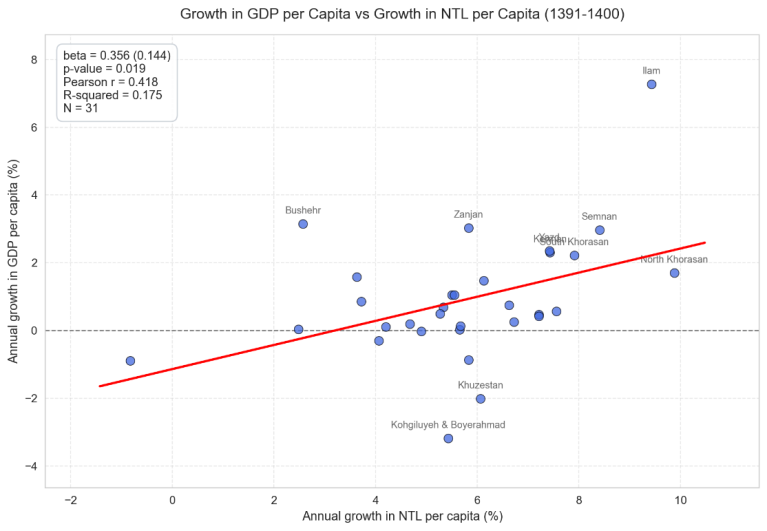
\includegraphics[width=\textwidth]{figs/growth.png}
\caption{Growth of GDP and radiance per capita, 1391--1400~SH.}
\label{fig:growth}
\end{subfigure}\hfill
\begin{subfigure}[t]{0.47\textwidth}
\centering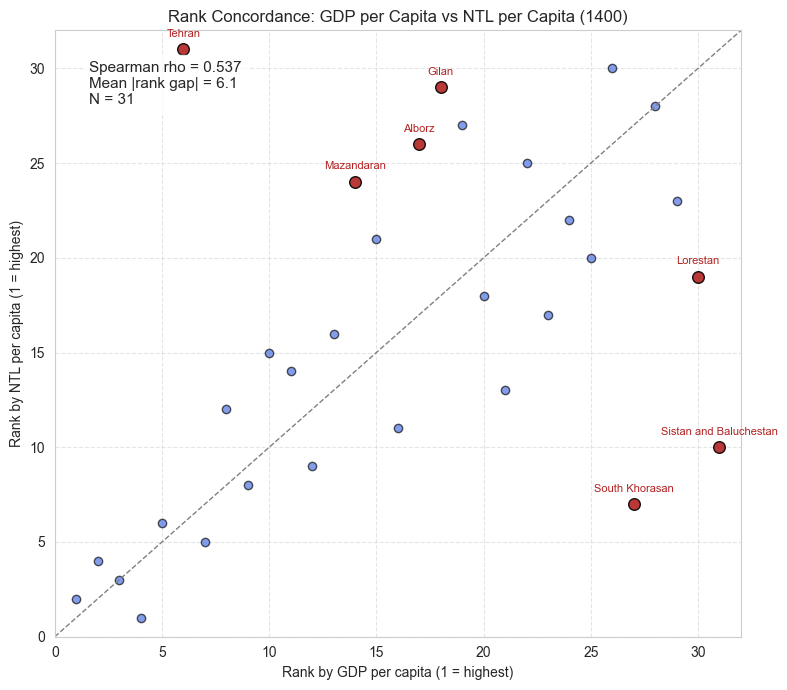
\includegraphics[width=\textwidth]{figs/rank.png}
\caption{Rank concordance, 1400~SH.}
\label{fig:rank}
\end{subfigure}
\caption{Provincial concordance between official GDP and nighttime lights.}
\label{fig:concord}
\end{figure}

The rank deviations are systematic rather than random. Dense provinces such as Tehran, Alborz and Gilan rank much lower by lights per capita than by GDP per capita, whereas sparsely populated provinces such as Sistan and Baluchestan and South Khorasan rank much higher (\cref{fig:rank}). Lights per capita therefore depend on population density as well as on activity. Because density is a persistent provincial characteristic, province fixed effects in the calibration absorb it; a direct comparison of per-capita levels without such adjustment would be misleading. The same insight bears on the city module, where lights per capita are compared across cities of very different density (\cref{sec:cities}).

\subsection{Two warnings and a first look at places versus people}\label{sec:prelimwarn}

Two further results from the preliminary work shape the design, and a third gives an early answer to RQ3.

\paragraph{A discontinuity in the light series}
Excluding the flaring provinces, light-based inequality jumps from 0.219 in 1395~SH to 0.289 in 1396~SH and stays near that level afterwards, while GDP- and expenditure-based inequality barely move in that year. A change of this size within one year would require a large shift in the relative position of provinces, and nothing in the economic data suggests one. The more likely explanations are a change in the satellite product or processing, or an error in mapping monthly composites to Solar years. I therefore do not interpret the post-1395 rise in light-based inequality as an economic result. The final series will be rebuilt from a single product version and the calendar mapping will be checked month by month (\cref{tab:threats}).

\paragraph{Lights and household welfare}
Lights rise in 30 of the 31 provinces over 1391--1403~SH, but real household expenditure per capita from the HIES falls in many of them. Within several provinces the correlation between the two series over time is strongly negative ($-0.78$ in East Azerbaijan, $-0.69$ in Kohgiluyeh and Boyer-Ahmad, $-0.63$ in Lorestan), while in others it is strongly positive (0.91 in Mazandaran, 0.88 in Tehran). In Iran, lights appear to follow infrastructure and electrification at least as closely as living standards. This is why the thesis uses lights to measure the location of \emph{activity} and keeps household data as the measure of \emph{welfare}.

\paragraph{Places and people already diverge}
Population-weighted inequality between provinces in real household expenditure rose steadily from about 0.16 in 1391~SH to 0.24 in 1403~SH, with a peak of 0.255 in 1402~SH. Over 1391--1400~SH, inequality in GDP per capita across the same provinces (excluding the flaring provinces) stayed between 0.22 and 0.24 with no clear trend. Output became no more concentrated, while the gap in what households in different provinces could spend widened. This is exactly the kind of divergence that RQ3 is designed to document over a longer period, and it motivates the decomposition of household inequality in \cref{sec:comparison}.

% =====================================================================
\section{Methodology}\label{sec:method}
% =====================================================================

\Cref{fig:pipeline} summarises the design. A common data infrastructure feeds two measurement modules, the provincial reconstruction and the satellite-defined city system, whose outputs are compared with interpersonal inequality.

\begin{figure}[htbp]
\centering
\resizebox{\textwidth}{!}{%
\begin{tikzpicture}[
  font=\sffamily\scriptsize,
  stage/.style={rectangle,rounded corners=2pt,draw=steel,fill=mist,text width=2.75cm,align=center,inner sep=4pt,minimum height=1.35cm},
  key/.style={stage,fill=navy,text=white,draw=navy},
  city/.style={stage,fill=sand,draw=rust!60},
  outbox/.style={stage,fill=white,draw=navy,line width=0.9pt},
  arr/.style={-{Stealth[length=2mm]},draw=steel,line width=0.7pt},
  lab/.style={font=\sffamily\bfseries\scriptsize,text=navy}]
% infrastructure
\node[stage] (raw) at (0,0) {\textbf{Data infrastructure}\\ lights (DMSP, \mbox{VIIRS}), flare masking, fixed 30-unit map, GDP, population};
% provincial
\node[key,right=0.5cm of raw,yshift=1.5cm] (cal) {\textbf{Calibration}\\ $\ln Y=\mu_i+\beta\ln L+\gamma t$\\ 1383--1401~SH};
\node[key,right=0.4cm of cal] (rec) {\textbf{Reconstruction}\\ backcast 1371--82\\ forecast 1402--03};
\node[stage,right=0.4cm of rec] (unc) {\textbf{Uncertainty}\\ parametric bootstrap\\ $\Rightarrow$ index bands};
% city
\node[city,right=0.5cm of raw,yshift=-1.5cm] (del) {\textbf{City delineation}\\ thresholds,\\ contiguity, VIIRS};
\node[city,right=0.4cm of del] (pop) {\textbf{Attributes}\\ lights, GHS-POP population, province};
\node[city,right=0.4cm of pop] (cidx) {\textbf{Urban system}\\ between-city inequality, decomposition, primacy};
% outputs
\node[outbox,right=0.5cm of unc,yshift=-1.5cm] (cmp) {\textbf{Comparison}\\ with national Gini: levels, differences, lags, turning points};
\draw[arr] (raw.east) -- ++(0.35,0) |- (cal.west);
\draw[arr] (raw.east) -- ++(0.35,0) |- (del.west);
\draw[arr] (cal) -- (rec); \draw[arr] (rec) -- (unc);
\draw[arr] (del) -- (pop); \draw[arr] (pop) -- (cidx);
\draw[arr] (unc.east) -- ++(0.35,0) |- (cmp.west);
\draw[arr] (cidx.east) -- ++(0.35,0) |- (cmp.west);
\node[stage,below=0.22cm of rec,fill=white,draw=rule,text width=2.75cm,minimum height=0.55cm,inner sep=2.5pt,font=\sffamily\tiny] (valid) {Validation: backcasting, flare and sensor tests, external comparator};
\draw[arr,dashed] (valid) -- (rec);
\node[lab,above=0.05cm of rec] {Provincial module (RQ1)};
\node[lab,below=0.05cm of pop,text=rust] {City module (RQ2)};
\node[lab,above=0.05cm of cmp] {RQ3};
\end{tikzpicture}}
\caption{Research design. Navy: provincial module; sand: city module.}
\label{fig:pipeline}
\end{figure}

\subsection{Measurement framework}\label{sec:framework}

Let $y^{*}_{it}$ denote the true log GDP of province $i$ in year $t$. Official statistics and lights each provide a noisy signal:
\begin{align}
y^{\text{off}}_{it} &= y^{*}_{it} + u_{it}, \label{eq:off}\\
\ln L_{it} &= a_i + b\,y^{*}_{it} + g\,t + e_{it}, \label{eq:lights}
\end{align}
where $u_{it}$ is the measurement error of official accounts and $e_{it}$ the noise in lights: differences in lighting technology and energy prices, flaring, sensor effects and the part of activity that emits no light. Equation~\eqref{eq:lights} allows the level of lights per unit of output to differ permanently across provinces ($a_i$), as the density pattern in \cref{fig:rank} requires, and to drift with technology ($g\,t$). Inverting \eqref{eq:lights} and substituting \eqref{eq:off} gives the estimable calibration equation of the next subsection; a light-based prediction of output can then be written as $\hat y_{it}=y^{*}_{it}+v_{it}$, with $v_{it}$ the prediction error.

\subsection{Calibration model}\label{sec:calibration}

Following \citet{LessmannSeidel2017}, adapted to a single-country panel, the calibration equation is estimated on the window $\mathcal{T}_c=\{1383,\ldots,1401\}$:
\begin{equation}
\ln Y_{it} = \mu_i + \beta \ln L_{it} + \gamma\, t + \varepsilon_{it}, \qquad i=1,\ldots,30,\; t\in\mathcal{T}_c,
\label{eq:calib}
\end{equation}
where $Y_{it}$ is official total GDP in constant prices and $L_{it}$ total flare-masked radiance. Three specification choices are deliberate.

\begin{itemize}
\item \emph{Province fixed effects} $\mu_i$ absorb persistent differences in the light--output ratio (density, sectoral structure, urban form). They are identified because every unit is present in every year on the fixed geography.
\item \emph{A linear trend instead of year fixed effects.} Year dummies cannot be extrapolated outside $\mathcal{T}_c$, whereas a trend can; it captures common drift in lighting efficiency and growth. Year fixed effects are used only in validation regressions.
\item \emph{Levels rather than per-capita values}, to avoid spurious correlation from a common population denominator.
\end{itemize}
Because $\ln L_{it}$ contains the noise $e_{it}$ of \eqref{eq:lights}, $\beta$ is a predictive (projection) coefficient rather than the structural inverse $1/b$; this is exactly what out-of-window prediction requires, and it is why validation is judged by predictive performance rather than by the size of $\hat\beta$.

Features of the original cross-country model of \citet{LessmannSeidel2017} (country-group and satellite fixed effects, the number of top-coded pixels and country area) were designed to predict output for countries with no regional data at all. In a single-country panel with fixed effects and VIIRS-quality data in most of the window, they are either unnecessary or not identified; their role is taken over by the diagnostics below.

\paragraph{Inference}
Errors are allowed to be heteroskedastic and serially correlated within provinces; standard errors are clustered by province. With only 30 clusters, inference uses the wild cluster bootstrap \citep{Cameron2008}.

\paragraph{Diagnostics}
Three assumptions behind \eqref{eq:calib} are tested rather than assumed.
\begin{enumerate}[label=(\alph*)]
\item \emph{Sensor regime.} Where the window spans the DMSP--VIIRS transition, the equation is augmented with a VIIRS indicator and its interaction with $\ln L_{it}$; a joint test of both coefficients is a test for a break at the splice. The calibration is also re-estimated on native-VIIRS years only (1391--1401~SH).
\item \emph{Slope homogeneity.} Province-specific slopes $\beta_i$ are estimated by the mean-group estimator \citep{PesaranSmith1995} and homogeneity is tested; heterogeneity is related to observable characteristics (density, oil share, region).
\item \emph{Flare contamination.} Results with pixel-level flare masking are compared with unmasked lights and with the exclusion of the four flaring provinces used in \cref{tab:provincial}.
\end{enumerate}

\subsection{Reconstruction: Dataset A (primary)}\label{sec:datasetA}

The fitted model generates GDP for every province-year in 1371--1403~SH:
\begin{equation}
\widehat{Y}_{it} = \hat s \cdot \exp\!\big(\hat\mu_i + \hat\beta \ln L_{it} + \hat\gamma\, t\big),
\qquad \hat s=\frac{1}{N}\sum_{j,\tau}\exp(\hat\varepsilon_{j\tau}),
\label{eq:predict}
\end{equation}
where $\hat s$ is the smearing factor of \citet{Duan1983}, which corrects the retransformation bias of predicting levels from a log model. Because $\hat s$ is common to all units, it cancels from every scale-invariant inequality index; it matters only when levels are reported.

\begin{keybox}[title={Why reconstruct the whole period, including years with official data?}]
In Dataset A, $\widehat{Y}_{it}$ replaces official GDP even inside the calibration window. This ensures that the entire series is produced by one method, so that any break or turning point in the inequality index cannot be an artefact of switching from official to predicted data. Official GDP plays the role of calibration and validation benchmark: inequality computed from official and from reconstructed GDP is compared year by year over 1383--1401~SH.
\end{keybox}

\subsection{Composite estimator: Dataset B (alternative)}\label{sec:datasetB}

The alternative dataset uses official data where available, improved by the information in lights. Within $\mathcal{T}_c$, the composite estimator of log GDP is
\begin{equation}
z_{it} = w\, y^{\text{off}}_{it} + (1-w)\,\hat y_{it},\qquad
w^{*}=\frac{\sigma^2_v}{\sigma^2_u+\sigma^2_v},
\label{eq:composite}
\end{equation}
where $\sigma^2_u=\Var(u_{it})$ and $\sigma^2_v=\Var(v_{it})$. If $u$ and $v$ are uncorrelated, $w^{*}$ minimises the error variance of $z$, which equals $\sigma^2_u\sigma^2_v/(\sigma^2_u+\sigma^2_v)$ and is smaller than either error variance alone \citep{ChenNordhaus2011,HendersonStoreygardWeil2012}. The noisier source receives less weight; as either variance tends to zero, its weight tends to one. Outside $\mathcal{T}_c$, $z_{it}=\hat y_{it}$.

\paragraph{Breaking the mechanical correlation}
Because $\hat y_{it}$ is fitted to official data, in-sample prediction errors are mechanically correlated with $u_{it}$, which violates the premise of \eqref{eq:composite}. Predictions entering the composite are therefore \emph{cross-fitted}: the value for year $t$ comes from a model estimated without year $t$. This removes the mechanical in-sample correlation, although persistent components of official error may remain, which is why Dataset B is the alternative rather than the primary series.

\paragraph{Identifying the error variances}
On within-province, detrended data (denoted by a tilde), and under uncorrelated errors with unit loadings,
\begin{equation}
\Cov(\tilde y^{\text{off}},\tilde{\hat y})=\Var(\tilde y^{*}),\quad
\sigma^2_u=\Var(\tilde y^{\text{off}})-\Cov(\tilde y^{\text{off}},\tilde{\hat y}),\quad
\sigma^2_v=\Var(\tilde{\hat y})-\Cov(\tilde y^{\text{off}},\tilde{\hat y}).
\label{eq:moments}
\end{equation}
Provincial electricity consumption provides a third indicator whose error is plausibly independent of both: used as an instrument for $\hat y$ in a regression of $y^{\text{off}}$ on $\hat y$, it identifies the relative loading of the two measures and provides an over-identification check on \eqref{eq:moments}. The gridded GDP of \citet{RossiHansbergZhang2025} is not suitable as a third indicator because it is itself predicted partly from lights; it is used only as an external comparator. Because these moments are imprecise in a short panel, results are also reported for a grid of weights $w\in[0,1]$, following the calibration logic of \citet{HendersonStoreygardWeil2012}.

The comparison of Datasets A and B is itself a result: similar inequality trajectories indicate robustness to the construction of the output measure, and divergences reveal where conclusions depend on it.

\subsection{Temporal validation}\label{sec:validation}

The reconstruction assumes that the relationship estimated in $\mathcal{T}_c$ holds outside it. This assumption is tested in three ways.
\begin{enumerate}[label=(\roman*)]
\item \emph{Backcasting.} The model is estimated on the later part of the window (e.g.\ 1392--1401~SH) and used to predict the earlier part (1383--1391~SH); root mean squared error and systematic bias are reported. This test mimics the actual task, prediction backwards in time, and is therefore more informative than random hold-outs.
\item \emph{Rolling windows.} The exercise is repeated for several estimation windows and forecast horizons, and the elasticity is compared across sub-periods defined by sensor regime and by macroeconomic episodes.
\item \emph{Index-level criterion.} The decisive criterion is not the accuracy of GDP predictions but the stability of the inequality index. Relative inequality indices are scale-invariant, so a prediction error common to all provinces leaves them unchanged; only errors that differ across provinces matter. In each validation window, the index is computed once from official and once from predicted GDP, and the two series are compared.
\end{enumerate}
If instability is detected, the specification is revised in the direction indicated by the pattern (e.g.\ sensor-specific slopes), and the revision is documented.

\subsection{Propagating reconstruction uncertainty}\label{sec:uncertainty}

Reconstructed values are estimates, and inequality indices built from them inherit their uncertainty. For $b=1,\ldots,B$ ($B=1{,}000$), parameters are drawn from their estimated sampling distribution, $\bm\theta^{(b)}\sim\mathcal{N}(\hat{\bm\theta},\hat{\bm V}_{\text{cl}})$, and residuals are resampled in province blocks to preserve serial correlation. Each draw yields a reconstructed panel $\widehat Y^{(b)}_{it}$ and an index series $I^{(b)}_t$. The 5th and 95th percentiles of $\{I^{(b)}_t\}$ give a 90 per cent band for every year. Bands are expected to widen with distance from $\mathcal{T}_c$, which makes the reliability of the backcast visible in every figure rather than relegating it to a footnote.

\subsection{Inequality indices}\label{sec:indices}

For units $i=1,\ldots,n$ with population shares $p_i$, per-capita output $y_i$ and population-weighted mean $\bar y=\sum_i p_i y_i$, the indices are
\begin{align}
G_w &= \frac{1}{2\bar y}\sum_{i=1}^{n}\sum_{j=1}^{n}p_i\,p_j\,\lvert y_i-y_j\rvert, \label{eq:gini}\\
GE(\alpha) &= \frac{1}{\alpha(\alpha-1)}\sum_{i=1}^{n}p_i\left[\left(\frac{y_i}{\bar y}\right)^{\alpha}-1\right],\qquad \alpha\neq 0,1, \label{eq:ge}\\
T &= GE(1)=\sum_{i}p_i\,\frac{y_i}{\bar y}\ln\frac{y_i}{\bar y},\qquad
MLD = GE(0)=\sum_{i}p_i\ln\frac{\bar y}{y_i}, \label{eq:theil}\\
CV_w &= \frac{1}{\bar y}\Big(\sum_i p_i (y_i-\bar y)^2\Big)^{1/2}. \label{eq:cv}
\end{align}
The population-weighted Gini \eqref{eq:gini} is the headline index because it is directly comparable with the national Gini; the Theil index and mean log deviation \eqref{eq:theil} are reported because they are additively decomposable, which is required in the city module; the weighted coefficient of variation \eqref{eq:cv} is Williamson's original measure. Population weighting is used throughout, so that indices measure inequality as experienced by the population rather than dispersion across administrative units; this is standard in the literature \citep{LessmannSeidel2017} and especially important in Iran, where provincial populations differ by a factor of more than twenty-five. Unweighted indices are reported as a robustness check.

\subsection{Satellite-defined cities}\label{sec:cities}

The city module answers RQ2 by measuring inequality across cities defined as economic rather than administrative entities. It deliberately uses no municipal or \emph{shahrestan} boundaries. The main analysis uses VIIRS (1391--1403~SH), whose resolution, dynamic range and absence of top-coding make it suitable for city footprints, whereas DMSP blooming systematically inflates urban extent \citep{Small2005,Gibson2025}. An extension back to 1383~SH uses the harmonised VIIRS-like series of \citet{ChenZ2021}, interpreted with corresponding caution.

\paragraph{Delineation algorithm}
\begin{enumerate}[label=\arabic*.]
\item \emph{Pre-processing.} Annual VIIRS composites with background noise removed are masked for gas flares (flare-site polygons, buffered) and water bodies before any thresholding, so that flaring sites cannot be mistaken for cities.
\item \emph{Thresholding.} Pixels with radiance above a threshold $\tau$ form a binary lit mask. Rather than imposing one value, a grid of thresholds is considered, as in \citet{Dingel2021}. The main threshold is chosen by out-of-sample agreement with an independent benchmark, the GHSL urban centres \citep{Dijkstra2021}, measured by spatial overlap (intersection over union).
\item \emph{Contiguity and clustering.} Lit pixels are grouped into 8-connected components. Components separated by a gap of at most $d$ km are merged, in the spirit of the City Clustering Algorithm \citep{Rozenfeld2011}, so that a city is not split by parks, rivers or highways; $d\in\{0,1,2\}$ is varied.
\item \emph{Filtering.} Clusters below a minimum population (e.g.\ 20{,}000 residents) or with implausibly low population density (industrial plants, ports, highway interchanges) are removed.
\item \emph{Time dimension.} The main specification fixes each city's footprint as the union of its lit area over the analysis period, so that inequality reflects changes in activity within constant territories; year-specific footprints, tracked across years by maximum spatial overlap, are a robustness check that captures spatial expansion and mergers.
\item \emph{Attributes.} For each city $c$ and year $t$: total radiance $L_{ct}$, population $P_{ct}$ from GHS-POP (interpolated log-linearly between epochs), area, lights per capita $\ell_{ct}=L_{ct}/P_{ct}$, and the province $k(c)$ containing the largest share of its footprint.
\end{enumerate}

\paragraph{Validation}
Footprints are compared with GHSL urban centres; footprint populations are compared with census city populations for 1385, 1390 and 1395~SH; and the rank--size relation is checked for plausibility. WorldPop is used only as a robustness check, because its population allocation uses nighttime lights as a covariate \citep{Stevens2015}, which would make lights per capita partly mechanical.

\needspace{5\baselineskip}
\paragraph{Analyses}
\begin{enumerate}[label=(\alph*)]
\item \emph{Between-city inequality.} The indices \eqref{eq:gini}--\eqref{eq:cv} are computed across cities for $\ell_{ct}$, weighted by city population, with uncertainty assessed over the threshold grid.
\item \emph{Decomposition across scales.} The Theil index across cities is decomposed into a between-province and a within-province component,
\begin{equation}
T^{\text{city}}_t = \underbrace{\sum_{k} s_{kt}\ln\frac{\bar\ell_{kt}}{\bar\ell_t}}_{\text{between provinces}} \;+\; \underbrace{\sum_{k} s_{kt}\,T_{kt}}_{\text{within provinces}},
\label{eq:decomp}
\end{equation}
where $s_{kt}$ is province $k$'s share of total urban lights, $\bar\ell_{kt}$ its mean urban lights per capita and $T_{kt}$ the Theil index across its cities. The between component links the city module to the provincial series; the within component measures intra-provincial urban disparities that the provincial analysis cannot see, which echoes the scale argument of \citet{LeeBreau2026}.
\item \emph{Urban primacy and city-size distribution.} The shares of Tehran and of the largest five cities in urban lights and population are tracked over time. The Pareto exponent of the city-size distribution is estimated with the rank$-\frac12$ estimator of \citet{GabaixIbragimov2011}, $\ln(R_c-\tfrac12)=\kappa-\zeta\ln P_c$, and its lights analogue with $L_c$ in place of $P_c$.
\end{enumerate}

\begin{notebox}[title={Interpretation of city-level results}]
No GDP exists at the city level, so the city module cannot be calibrated and its results describe the spatial distribution of \emph{urban} activity as revealed by light, not output. Two features make it informative nonetheless. First, the cross-sectional elasticity of provincial GDP with respect to lights is close to one (\cref{tab:provincial}), which implies that cross-sectional shares of lights approximate shares of activity. Second, defining cities by their footprint removes the arbitrariness of administrative boundaries that \citet{Magrini2004} and \citet{Dingel2021} show can drive results. Because lights per capita also reflect density (\cref{sec:prelimprov}), city comparisons are reported both in levels and conditional on density.
\end{notebox}

\subsection{Comparing spatial and interpersonal inequality}\label{sec:comparison}

Let $S_t$ denote a spatial-inequality index (provincial, 1371--1403~SH; city-based, 1391--1403~SH) and $G_t$ the national Gini. The comparison has five components.
\begin{enumerate}[label=(\roman*)]
\item \emph{Correlation in levels and in first differences.} Correlation in levels can merely reflect common trends; first differences reduce the risk of spurious correlation. Augmented Dickey--Fuller tests are reported for information, recognising their low power with about 33 annual observations.
\item \emph{Co-movement regression.}
\begin{equation}
\Delta S_t = \alpha + \delta\,\Delta G_t + \eta_t,
\label{eq:comove}
\end{equation}
with Newey--West standard errors \citep{NeweyWest1987}. A positive and significant $\delta$ indicates co-movement; its sign and size are descriptive, not causal.
\item \emph{Lead--lag structure.} Cross-correlations of $\Delta S_t$ and $\Delta G_{t+k}$ for $k=-3,\ldots,3$ examine whether movements in one dimension precede movements in the other.
\item \emph{Turning points and episodes.} Turning points of both series are dated and compared with the episodes in \cref{tab:mechanisms}: the 1389~SH subsidy reform and the sanctions shocks of 1390--91 and 1397~SH. Reconstruction uncertainty bands (\cref{sec:uncertainty}) indicate which movements in $S_t$ are distinguishable from measurement noise.
\item \emph{Decomposing household inequality by province.} Using the HIES microdata, the Theil index and mean log deviation of household expenditure are decomposed each year into a between-province and a within-province component. The between-province component is a people-based counterpart of $S_t$, measured on the same households as the national Gini, and the within-province component shows how much of the national movement happens inside provinces. Comparing $S_t$ with this between-province component separates two questions that the national Gini mixes: whether output and welfare diverge across places, and whether inequality among households changes within places.
\end{enumerate}
In interpreting results, the conceptual difference between the two measures is kept explicit: the national Gini aggregates between- and within-province inequality among households, whereas $S_t$ measures only between-unit inequality in average activity. The comparison therefore focuses on directions, turning points and periods of co-movement, not on levels.

% =====================================================================
\section{Validity, Robustness and Limitations}\label{sec:validity}
% =====================================================================

\subsection{Threats to validity}

\Cref{tab:threats} lists the main threats and the strategy for each.

\begin{table}[htbp]
\centering\small
\caption{Threats to validity and responses}
\label{tab:threats}
\begin{tabularx}{\textwidth}{@{}>{\raggedright\arraybackslash}p{3.6cm}>{\raggedright\arraybackslash}X@{}}
\toprule
\textbf{Threat} & \textbf{Response}\\
\midrule
Reconstruction error grows with distance from the calibration window & Backcasting and rolling-window validation (\cref{sec:validation}); bootstrap bands on every index (\cref{sec:uncertainty}); results shown separately for the calibration window and the reconstructed years.\\
\addlinespace
Weak within-province temporal signal & Longer, 19-year window; index-level validation; explicit report of fixed-effects elasticities (\cref{tab:provincial}); \citet{Galimberti2023} distinction between cross-sectional and temporal validity.\\
\addlinespace
Gas-flare contamination & Pixel-level masking with flare-site data before aggregation and before city delineation; comparison with exclusion of flaring provinces.\\
\addlinespace
Sensor change (DMSP to VIIRS) & Harmonised series; sensor-break test; re-estimation on VIIRS-only years; all main results repeated for the VIIRS period.\\
\addlinespace
Heterogeneous light--output relationship & Province fixed effects; mean-group slopes and homogeneity test; analysis of residuals by density, oil share and region.\\
\addlinespace
Boundary changes & Fixed 30-unit geography (post-1383 map, Tehran and Alborz merged); lights summed over fixed polygons.\\
\addlinespace
Arbitrary city definition & Threshold and merging-distance grids; benchmark-based threshold choice; fixed and time-varying footprints.\\
\addlinespace
Population data built from lights & GHS-POP (built-up based) as main source; WorldPop only for robustness.\\
\addlinespace
Attenuation in the reconstruction & With $\hat\beta<1$, reconstructed changes in relative GDP are damped versions of changes in relative lights, so the backcast will tend to make inequality look flatter than it was. The lights-only index is reported alongside, $\beta$ is also estimated on long differences, and flat segments of the backcast are interpreted with caution.\\
\addlinespace
Product and processing discontinuities & The 1395$\to$1396~SH jump in light-based inequality (\cref{sec:prelimwarn}): series rebuilt from a single product version; month-by-month check of the Solar-calendar mapping; comparison with GDP and expenditure in the same years.\\
\addlinespace
Changes in lighting technology & The VIIRS sensor is largely blind to the blue part of LED light \citep{Kyba2017}, so a switch to LED street lighting can lower measured radiance in large cities without any fall in activity. Province-specific trends are tested as a robustness check, and large cities are flagged in the city module.\\
\bottomrule
\end{tabularx}
\end{table}

\subsection{Pre-specified robustness checks}

The following checks are specified before the final results are observed, to avoid selective reporting:
\begin{enumerate}[label=\arabic*.]
\item All indices: Gini, Theil, mean log deviation and weighted coefficient of variation; weighted and unweighted.
\item Dataset A versus Dataset B, and Dataset B over a grid of weights.
\item Backcasting test (estimate on 1392--1401, predict 1383--1391~SH), with RMSE and bias for GDP and for the inequality index.
\item Calibration on native-VIIRS years only, and with sensor-specific slopes.
\item Flare masking versus exclusion of the four flaring provinces; exclusion of provinces with extreme residuals.
\item Total versus non-oil GDP as the calibration target.
\item For cities: threshold grid, merging distance, minimum size, fixed versus time-varying footprints, GHS-POP versus WorldPop.
\end{enumerate}

\subsection{Limitations}

\paragraph{Descriptive, not causal}
The thesis documents co-movement and divergence between the two dimensions of inequality; it does not identify causal effects between them. This limitation is accepted deliberately: the research question is about how the two dimensions evolved, and answering it does not require a causal estimate. Co-movement analysis alone cannot separate the mechanisms in \cref{tab:mechanisms}; doing so would require event-specific designs (\cref{sec:extensions}).

\paragraph{Limited time-series length}
About 33 annual observations constrain the power of time-series tests. Extending the period to 1371~SH increases the number of observations, at the cost of relying on reconstructed values; the trade-off is made explicit through uncertainty bands.

\paragraph{Scale}
The provincial index captures only between-province inequality, which the literature shows to be a minority of total inequality. The city module partly addresses this by revealing within-province urban disparities, but rural areas lie outside it by construction.

\paragraph{External validity}
Iran is an oil-dependent economy with a centralised institutional structure and repeated external shocks; findings may not generalise to economies with different structures. The measurement approach, however, is portable.

\paragraph{Fallback}
If harmonisation of pre-VIIRS lights proves unreliable, the core of the thesis (the comparison of the two dimensions over the calibration window and the VIIRS-based city system) remains intact, and the long backcast is presented as an extension.

% =====================================================================
\section{Expected Contributions and Work Plan}\label{sec:contrib}
% =====================================================================

\subsection{Contributions}

\begin{keybox}[title={Expected contributions}]
\begin{enumerate}[label=\arabic*.,leftmargin=1.2em]
\item \textbf{Data.} To the author's knowledge, the first consistent series of interprovincial inequality in economic activity for Iran, 1371--1403~SH, on a fixed geography, with official GDP as anchor and quantified reconstruction uncertainty.
\item \textbf{Measurement.} An application of the measurement-error framework of \citet{ChenNordhaus2011} and \citet{HendersonStoreygardWeil2012} to regional inequality in Iran, with cross-fitting to address the mechanical correlation between official and calibrated light-based output, and propagation of uncertainty into inequality indices.
\item \textbf{Cities.} The first delineation of Iran's urban system from space, independent of administrative boundaries, with between-city inequality decomposed across spatial scales and the evolution of urban primacy.
\item \textbf{Substance.} Systematic evidence on whether spatial and interpersonal inequality in Iran moved together or apart, and when. This evidence bears on the evaluation of people-based and place-based policies.
\end{enumerate}
\end{keybox}

\subsection{Extensions: using the distinction}\label{sec:extensions}

The distinction between the two dimensions has practical value because policies affect them differently. Once the series exist, three episodes offer natural extensions, beyond the scope of the thesis itself. (i) The 1389~SH subsidy reform: universal cash transfers should reduce interpersonal inequality without necessarily changing the geography of production. (ii) Sanctions: exposure through foreign trade, customs and export industries is spatially concentrated, so their effect should be more visible in spatial than in interpersonal inequality. (iii) Deprivation-reduction and provincial development budgets: these are place-based by design, so their effect should appear in spatial inequality even if it is invisible in the national Gini. Each would require its own identification strategy.

\subsection{Work plan}

\begin{table}[htbp]
\centering\small
\caption{Work plan}
\label{tab:plan}
\begin{tabularx}{\textwidth}{@{}c>{\raggedright\arraybackslash}p{3.7cm}>{\raggedright\arraybackslash}X@{}}
\toprule
\textbf{Phase} & \textbf{Task} & \textbf{Deliverable}\\
\midrule
\textsf{\textbf{\color{navy}1}} & Data infrastructure & Fixed 30-unit polygons; flare-masked lights 1371--1403~SH; harmonised sensor series; assembled panel with GDP, population and electricity.\\
\textsf{\textbf{\color{navy}2}} & Calibration and validation & Estimates of \eqref{eq:calib}; sensor, slope and flare diagnostics; backcasting and rolling-window results.\\
\textsf{\textbf{\color{navy}3}} & Reconstruction and indices & Datasets A and B; inequality indices 1371--1403~SH with bootstrap bands.\\
\textsf{\textbf{\color{navy}4}} & City module & City footprints and validation; between-city inequality, decomposition and primacy, 1391--1403~SH; extension to 1383~SH.\\
\textsf{\textbf{\color{navy}5}} & Comparison and writing & Co-movement analysis; thesis chapters; journal-article draft.\\
\bottomrule
\end{tabularx}
\end{table}

% =====================================================================
%  REFERENCES
% =====================================================================
\newpage
\phantomsection
\addcontentsline{toc}{section}{References}
\begin{thebibliography}{99}

\bibitem[Abounoori et~al.(2013)]{Abounoori2013}
Abounoori, Esmaiel, Arash Khoshkar, and Pedram Davoudi. 2013. ``Decomposition of the Gini Coefficient in Iran by Urban and Rural Areas.'' \textit{Journal of Economic Research (Tahghighat-e Eghtesadi)} 48 (3): 1--21. (In Persian.)

\bibitem[Abrahams et~al.(2018)]{Abrahams2018}
Abrahams, Alexei, Christopher Oram, and Nancy Lozano-Gracia. 2018. ``Deblurring DMSP Nighttime Lights: A New Method Using Gaussian Filters and Frequencies of Illumination.'' \textit{Remote Sensing of Environment} 210: 242--258.

\bibitem[Ahmadi et~al.(2019)]{Ahmadi2019}
Ahmadi, Marzieh, Ali Falahati, and Sohrab Delangizan. 2019. ``Transition Dynamic Analysis of the Regional Disparity in Iran (Case Study: Iran Provinces).'' \textit{Quarterly Journal of Quantitative Economics} 16 (1): 97--113. (In Persian.)

\bibitem[Alonso(1980)]{Alonso1980}
Alonso, William. 1980. ``Five Bell Shapes in Development.'' \textit{Papers of the Regional Science Association} 45 (1): 5--16.

\bibitem[Amos(1988)]{Amos1988}
Amos, Orley M. 1988. ``Unbalanced Regional Growth and Regional Income Inequality in the Latter Stages of Development.'' \textit{Regional Science and Urban Economics} 18 (4): 549--566.

\bibitem[Azam and Bhatt(2018)]{AzamBhatt2018}
Azam, Mehtabul, and Vipul Bhatt. 2018. ``Spatial Income Inequality in India, 1993--2011: A Decomposition Analysis.'' \textit{Social Indicators Research} 138 (2): 505--522.

\bibitem[Baragwanath et~al.(2021)]{Baragwanath2021}
Baragwanath, Kathryn, Ran Goldblatt, Gordon Hanson, and Amit K. Khandelwal. 2021. ``Detecting Urban Markets with Satellite Imagery: An Application to India.'' \textit{Journal of Urban Economics} 125: 103173.

\bibitem[Bluhm and Krause(2022)]{Bluhm2022}
Bluhm, Richard, and Melanie Krause. 2022. ``Top Lights: Bright Cities and Their Contribution to Economic Development.'' \textit{Journal of Development Economics} 157: 102880.

\bibitem[Cameron et~al.(2008)]{Cameron2008}
Cameron, A. Colin, Jonah B. Gelbach, and Douglas L. Miller. 2008. ``Bootstrap-Based Improvements for Inference with Clustered Errors.'' \textit{Review of Economics and Statistics} 90 (3): 414--427.

\bibitem[Capello and Cerisola(2024)]{CapelloCerisola2024}
Capello, Roberta, and Silvia Cerisola. 2024. ``Towards a Double Bell Theory of Regional Disparities.'' \textit{Annals of Regional Science} 73 (4): 1701--1728.

\bibitem[Ch et~al.(2021)]{ChMartinVargas2021}
Ch, Rafael, Diego A. Martin, and Juan F. Vargas. 2021. ``Measuring the Size and Growth of Cities Using Nighttime Light.'' \textit{Journal of Urban Economics} 125: 103254.

\bibitem[Chen and Nordhaus(2011)]{ChenNordhaus2011}
Chen, Xi, and William D. Nordhaus. 2011. ``Using Luminosity Data as a Proxy for Economic Statistics.'' \textit{Proceedings of the National Academy of Sciences} 108 (21): 8589--8594.

\bibitem[Chen et~al.(2021)]{ChenZ2021}
Chen, Zuoqi, Bailang Yu, Chengshu Yang, Yuyu Zhou, Shenjun Yao, Xingjian Qian, Congxiao Wang, Bin Wu, and Jianping Wu. 2021. ``An Extended Time Series (2000--2018) of Global NPP-VIIRS-like Nighttime Light Data from a Cross-Sensor Calibration.'' \textit{Earth System Science Data} 13: 889--906.

\bibitem[de~Bellefon et~al.(2021)]{deBellefon2021}
de~Bellefon, Marie-Pierre, Pierre-Philippe Combes, Gilles Duranton, Laurent Gobillon, and Cl\'ement Gorin. 2021. ``Delineating Urban Areas Using Building Density.'' \textit{Journal of Urban Economics} 125: 103226.

\bibitem[Dehghan~Shabani et~al.(2019)]{DehghanShabani2019}
Dehghan~Shabani, Zahra, Ebrahim Hadian, and Jamal Negahdari. 2019. ``Analysis of the Relationship between Regional Inequality and Economic Development in Iran: Spatial Dynamic Panel Data Approach.'' \textit{Journal of Economic Research (Tahghighat-e Eghtesadi)} 54 (4): 875--890. (In Persian.)

\bibitem[Dijkstra et~al.(2021)]{Dijkstra2021}
Dijkstra, Lewis, Aneta J. Florczyk, Sergio Freire, Thomas Kemper, Michele Melchiorri, Martino Pesaresi, and Marcello Schiavina. 2021. ``Applying the Degree of Urbanisation to the Globe: A New Harmonised Definition Reveals a Different Picture of Global Urbanisation.'' \textit{Journal of Urban Economics} 125: 103312.

\bibitem[Dingel et~al.(2021)]{Dingel2021}
Dingel, Jonathan I., Antonio Miscio, and Donald R. Davis. 2021. ``Cities, Lights, and Skills in Developing Economies.'' \textit{Journal of Urban Economics} 125: 103174.

\bibitem[Duan(1983)]{Duan1983}
Duan, Naihua. 1983. ``Smearing Estimate: A Nonparametric Retransformation Method.'' \textit{Journal of the American Statistical Association} 78 (383): 605--610.

\bibitem[Elvidge et~al.(2016)]{Elvidge2016}
Elvidge, Christopher D., Mikhail Zhizhin, Kimberly Baugh, Feng-Chi Hsu, and Tilottama Ghosh. 2016. ``Methods for Global Survey of Natural Gas Flaring from Visible Infrared Imaging Radiometer Suite Data.'' \textit{Energies} 9 (1): 14.

\bibitem[Elvidge et~al.(2021)]{Elvidge2021}
Elvidge, Christopher D., Mikhail Zhizhin, Tilottama Ghosh, Feng-Chi Hsu, and Jay Taneja. 2021. ``Annual Time Series of Global VIIRS Nighttime Lights Derived from Monthly Averages: 2012 to 2019.'' \textit{Remote Sensing} 13 (5): 922.

\bibitem[Farzanegan and Fischer(2021)]{FarzaneganFischer2021}
Farzanegan, Mohammad Reza, and Sven Fischer. 2021. ``Lifting of International Sanctions and the Shadow Economy in Iran---A View from Outer Space.'' \textit{Remote Sensing} 13 (22): 4620.

\bibitem[Fouladgar and Feizi(2023)]{FouladgarFeizi2023}
Fouladgar, Vahid, and Mehdi Feizi. 2023. ``Estimation of Iran's Seasonal GDP Using Night Light Images.'' \textit{Journal of Economics and Regional Development} 29 (24). doi:10.22067/erd.2023.77085.1127. (In Persian.)

\bibitem[Fratesi and Percoco(2014)]{Fratesi2014}
Fratesi, Ugo, and Marco Percoco. 2014. ``Selective Migration, Regional Growth and Convergence: Evidence from Italy.'' \textit{Regional Studies} 48 (10): 1650--1668.

\bibitem[Gabaix and Ibragimov(2011)]{GabaixIbragimov2011}
Gabaix, Xavier, and Rustam Ibragimov. 2011. ``Rank$-$1/2: A Simple Way to Improve the OLS Estimation of Tail Exponents.'' \textit{Journal of Business \& Economic Statistics} 29 (1): 24--39.

\bibitem[Galimberti et~al.(2023)]{Galimberti2023}
Galimberti, Jaqueson K., Stefan Pichler, and Regina Pleninger. 2023. ``Measuring Inequality Using Geospatial Data.'' \textit{World Bank Economic Review} 37 (4): 549--569.

\bibitem[Gibson et~al.(2021)]{Gibson2021}
Gibson, John, Susan Olivia, Geua Boe-Gibson, and Chao Li. 2021. ``Which Night Lights Data Should We Use in Economics, and Where?'' \textit{Journal of Development Economics} 149: 102602.

\bibitem[Gibson et~al.(2025)]{Gibson2025}
Gibson, John, Olivia Alimi, and Geua Boe-Gibson. 2025. ``Lost in Translation? A Critical Review of Economics Research Using Nighttime Lights Data.'' \textit{Remote Sensing} 17 (7): 1130.

\bibitem[Hadizadeh(2020)]{Hadizadeh2020}
Hadizadeh, Arash. 2020. ``Income Inequality Convergence among Iran's Provinces: Finding New Evidence Using Parametric and Nonparametric Approaches.'' \textit{Iranian Economic Review} 24: 907--921.

\bibitem[Harari(2020)]{Harari2020}
Harari, Mariaflavia. 2020. ``Cities in Bad Shape: Urban Geometry in India.'' \textit{American Economic Review} 110 (8): 2377--2421.

\bibitem[Henderson et~al.(2012)]{HendersonStoreygardWeil2012}
Henderson, J. Vernon, Adam Storeygard, and David N. Weil. 2012. ``Measuring Economic Growth from Outer Space.'' \textit{American Economic Review} 102 (2): 994--1028.

\bibitem[Imhoff et~al.(1997)]{Imhoff1997}
Imhoff, Marc L., William T. Lawrence, David C. Stutzer, and Christopher D. Elvidge. 1997. ``A Technique for Using Composite DMSP/OLS `City Lights' Satellite Data to Map Urban Area.'' \textit{Remote Sensing of Environment} 61 (3): 361--370.

\bibitem[Ivan et~al.(2020)]{Ivan2020}
Ivan, Kinga, Iulian-Horia Holob\^ac\u{a}, J\'ozsef Benedek, and Ibolya T\"or\"ok. 2020. ``Potential of Night-Time Lights to Measure Regional Inequality.'' \textit{Remote Sensing} 12 (1): 33.

\bibitem[Khan and Siddique(2021)]{KhanSiddique2021}
Khan, Muhammad Salar, and Abu Bakkar Siddique. 2021. ``Spatial Analysis of Regional and Income Inequality in the United States.'' \textit{Economies} 9 (4): 159.

\bibitem[Krugman(1991)]{Krugman1991}
Krugman, Paul. 1991. ``Increasing Returns and Economic Geography.'' \textit{Journal of Political Economy} 99 (3): 483--499.

\bibitem[Kuznets(1955)]{Kuznets1955}
Kuznets, Simon. 1955. ``Economic Growth and Income Inequality.'' \textit{American Economic Review} 45 (1): 1--28.

\bibitem[Kyba et~al.(2017)]{Kyba2017}
Kyba, Christopher C.\,M., Theres Kuester, Alejandro S\'anchez de~Miguel, Kimberly Baugh, Andreas Jechow, Franz H\"olker, Jonathan Bennie, Christopher D. Elvidge, Kevin J. Gaston, and Luis Guanter. 2017. ``Artificially Lit Surface of Earth at Night Increasing in Radiance and Extent.'' \textit{Science Advances} 3 (11): e1701528.

\bibitem[Lee and Breau(2026)]{LeeBreau2026}
Lee, Annie S., and S\'ebastien Breau. 2026. ``Scales of Inequality: Applying a Two-Stage Theil Decomposition Approach to Examine the Changing Spatial Dimensions of Regional Inequality in the US, 1970--2020.'' \textit{International Regional Science Review}, online first. doi:10.1177/01600176261440842.

\bibitem[Lessmann(2014)]{Lessmann2014}
Lessmann, Christian. 2014. ``Spatial Inequality and Development---Is There an Inverted-U Relationship?'' \textit{Journal of Development Economics} 106: 35--51.

\bibitem[Lessmann and Seidel(2017)]{LessmannSeidel2017}
Lessmann, Christian, and Andr\'e Seidel. 2017. ``Regional Inequality, Convergence, and Its Determinants---A View from Outer Space.'' \textit{European Economic Review} 92: 110--132.

\bibitem[Leyk et~al.(2019)]{Leyk2019}
Leyk, Stefan, Andrea E. Gaughan, Susana B. Adamo, Alex de~Sherbinin, Deborah Balk, Sergio Freire, Amy Rose, Forrest R. Stevens, Brian Blankespoor, Charlie Frye, Joshua Comenetz, Alessandro Sorichetta, Kytt MacManus, Linda Pistolesi, Marc Levy, Andrew J. Tatem, and Martino Pesaresi. 2019. ``The Spatial Allocation of Population: A Review of Large-Scale Gridded Population Data Products and Their Fitness for Use.'' \textit{Earth System Science Data} 11: 1385--1409.

\bibitem[Li et~al.(2020)]{Li2020}
Li, Xuecao, Yuyu Zhou, Min Zhao, and Xia Zhao. 2020. ``A Harmonized Global Nighttime Light Dataset 1992--2018.'' \textit{Scientific Data} 7: 168.

\bibitem[Magrini(2004)]{Magrini2004}
Magrini, Stefano. 2004. ``Regional (Di)Convergence.'' In \textit{Handbook of Regional and Urban Economics}, Vol.\ 4, edited by J.~Vernon Henderson and Jacques-Fran\c{c}ois Thisse, 2741--2796. Amsterdam: Elsevier.

\bibitem[Mirza et~al.(2021)]{Mirza2021}
Mirza, M. Usman, Chi Xu, Bas van Bavel, Egbert H. van Nes, and Marten Scheffer. 2021. ``Global Inequality Remotely Sensed.'' \textit{Proceedings of the National Academy of Sciences} 118 (18): e1919913118.

\bibitem[Montalvo et~al.(2021)]{Montalvo2021}
Montalvo, Jos\'e G., Marta Reynal-Querol, and Juan Carlos Mu\~noz-Mora. 2021. ``Measuring Inequality from Above.'' Barcelona GSE Working Paper 1252.

\bibitem[Mveyange(2015)]{Mveyange2015}
Mveyange, Anthony. 2015. ``Night Lights and Regional Income Inequality in Africa.'' WIDER Working Paper 2015/085. Helsinki: UNU-WIDER.

\bibitem[Newey and West(1987)]{NeweyWest1987}
Newey, Whitney K., and Kenneth D. West. 1987. ``A Simple, Positive Semi-Definite, Heteroskedasticity and Autocorrelation Consistent Covariance Matrix.'' \textit{Econometrica} 55 (3): 703--708.

\bibitem[Noorbakhsh(2005)]{Noorbakhsh2005}
Noorbakhsh, Farhad. 2005. ``Spatial Inequality, Polarisation and Its Dimensions in Iran: New Empirical Evidence.'' \textit{Oxford Development Studies} 33 (3--4): 473--491.

\bibitem[Novotn\'y(2007)]{Novotny2007}
Novotn\'y, Josef. 2007. ``On the Measurement of Regional Inequality: Does Spatial Dimension of Income Inequality Matter?'' \textit{Annals of Regional Science} 41 (3): 563--580.

\bibitem[Pesaran and Smith(1995)]{PesaranSmith1995}
Pesaran, M. Hashem, and Ron Smith. 1995. ``Estimating Long-Run Relationships from Dynamic Heterogeneous Panels.'' \textit{Journal of Econometrics} 68 (1): 79--113.

\bibitem[Pesaresi et~al.(2024)]{Pesaresi2024}
Pesaresi, Martino, Marcello Schiavina, Panagiotis Politis, Sergio Freire, Katarzyna Krasnod\k{e}bska, Johannes H. Uhl, Alessandra Carioli, et~al. 2024. ``Advances on the Global Human Settlement Layer by Joint Assessment of Earth Observation and Population Survey Data.'' \textit{International Journal of Digital Earth} 17 (1): 2390454.

\bibitem[Pinkovskiy and Sala-i-Martin(2016)]{PinkovskiySalaiMartin2016}
Pinkovskiy, Maxim, and Xavier Sala-i-Martin. 2016. ``Lights, Camera\ldots{} Income! Illuminating the National Accounts--Household Surveys Debate.'' \textit{Quarterly Journal of Economics} 131 (2): 579--631.

\bibitem[Pourfaraj et~al.(2019)]{Pourfaraj2019}
Pourfaraj, Alireza, Nader Mehregan, Saeed Karimi Potanlar, and Mohammad Reza Eskandariata. 2019. ``Regional Inequality in Iran and the Impact of Economic Factors: A Spatial Econometric Approach.'' \textit{Iranian Economic Review} 23 (2): 297--318.

\bibitem[Rey(2018)]{Rey2018}
Rey, Sergio J. 2018. ``Bells in Space: The Spatial Dynamics of US Interpersonal and Interregional Income Inequality.'' \textit{International Regional Science Review} 41 (2): 152--182.

\bibitem[Rossi-Hansberg and Zhang(2025)]{RossiHansbergZhang2025}
Rossi-Hansberg, Esteban, and Jialing Zhang. 2025. ``Local GDP Estimates Around the World.'' NBER Working Paper 33458.

\bibitem[Rozenfeld et~al.(2008)]{Rozenfeld2008}
Rozenfeld, Hern\'an D., Diego Rybski, Jos\'e S. Andrade, Michael Batty, H. Eugene Stanley, and Hern\'an A. Makse. 2008. ``Laws of Population Growth.'' \textit{Proceedings of the National Academy of Sciences} 105 (48): 18702--18707.

\bibitem[Rozenfeld et~al.(2011)]{Rozenfeld2011}
Rozenfeld, Hern\'an D., Diego Rybski, Xavier Gabaix, and Hern\'an A. Makse. 2011. ``The Area and Population of Cities: New Insights from a Different Perspective on Cities.'' \textit{American Economic Review} 101 (5): 2205--2225.

\bibitem[Schiavina et~al.(2023)]{Schiavina2023}
Schiavina, Marcello, Sergio Freire, Alessandra Carioli, and Kytt MacManus. 2023. ``GHS-POP R2023A: GHS Population Grid Multitemporal (1975--2030).'' European Commission, Joint Research Centre. doi:10.2905/2FF68A52-5B5B-4A22-8F40-C41DA8332CFE.

\bibitem[Shorrocks and Wan(2005)]{Shorrocks2005}
Shorrocks, Anthony, and Guanghua Wan. 2005. ``Spatial Decomposition of Inequality.'' \textit{Journal of Economic Geography} 5 (1): 59--81.

\bibitem[Singhal et~al.(2020)]{Singhal2020}
Singhal, Abhishek, Sohini Sahu, Siddhartha Chattopadhyay, Abhijit Mukherjee, and Soumendra N. Bhanja. 2020. ``Using Night Time Lights to Find Regional Inequality in India and Its Relationship with Economic Development.'' \textit{PLOS ONE} 15 (11): e0241907.

\bibitem[Small et~al.(2005)]{Small2005}
Small, Christopher, Francesca Pozzi, and Christopher D. Elvidge. 2005. ``Spatial Analysis of Global Urban Extent from DMSP-OLS Night Lights.'' \textit{Remote Sensing of Environment} 96 (3--4): 277--291.

\bibitem[Stevens et~al.(2015)]{Stevens2015}
Stevens, Forrest R., Andrea E. Gaughan, Catherine Linard, and Andrew J. Tatem. 2015. ``Disaggregating Census Data for Population Mapping Using Random Forests with Remotely-Sensed and Ancillary Data.'' \textit{PLOS ONE} 10 (2): e0107042.

\bibitem[Weidmann and Schutte(2017)]{WeidmannSchutte2017}
Weidmann, Nils B., and Sebastian Schutte. 2017. ``Using Night Light Emissions for the Prediction of Local Wealth.'' \textit{Journal of Peace Research} 54 (2): 125--140.

\bibitem[Weidmann and Theunissen(2021)]{WeidmannTheunissen2021}
Weidmann, Nils B., and Gerlinde Theunissen. 2021. ``Estimating Local Inequality from Nighttime Lights.'' \textit{Remote Sensing} 13 (22): 4624.

\bibitem[Williamson(1965)]{Williamson1965}
Williamson, Jeffrey G. 1965. ``Regional Inequality and the Process of National Development: A Description of the Patterns.'' \textit{Economic Development and Cultural Change} 13 (4, Part 2): 1--84.

\bibitem[Wu et~al.(2018)]{Wu2018}
Wu, Rongwei, Degang Yang, Jiefang Dong, Lu Zhang, and Fuqiang Xia. 2018. ``Regional Inequality in China Based on NPP-VIIRS Night-Time Light Imagery.'' \textit{Remote Sensing} 10 (2): 240.

\bibitem[Zhou et~al.(2014)]{Zhou2014}
Zhou, Yuyu, Steven J. Smith, Christopher D. Elvidge, Kaiguang Zhao, Allison Thomson, and Marc Imhoff. 2014. ``A Cluster-Based Method to Map Urban Area from DMSP/OLS Nightlights.'' \textit{Remote Sensing of Environment} 147: 173--185.

\end{thebibliography}

\end{document}
